%
% supplement.tex -- Supplement zur Vorlesung Lineare Algebra
%                   gehalten an der Hochschule Rapperswil im Wintersemester 17
%
% (c) 2017 Prof. Dr. Andreas Mueller, HSR
%
\documentclass{book}
\usepackage{german}
\usepackage[utf8]{inputenc}
\usepackage{times}
\usepackage{amsmath}
\usepackage{amssymb}
\usepackage{amsfonts}
\usepackage{amsthm}
\usepackage{graphicx}
\usepackage{fancyhdr}
\usepackage{textcomp}
\usepackage[all]{xy}
\usepackage{txfonts}
\usepackage{array}
\usepackage{makeidx}
\usepackage{verbatim}
\usepackage{pdflscape}
\usepackage{paralist}
\usepackage{stmaryrd}
\usepackage{epic}
\usepackage[colorlinks=true]{hyperref}
\usepackage{geometry}
\geometry{papersize={170mm,240mm},total={140mm,200mm},top=21mm,bindingoffset=10mm}
\setlength{\unitlength}{1pt}
\usepackage{color}
\usepackage{enumitem}
\input ../skript/linsys.tex
\makeindex
\setlength{\headheight}{15pt}
\begin{document}
\pagestyle{fancy}
\lhead{Tabea's Supplement}
\frontmatter
\newcommand\HRule{\noindent\rule{\linewidth}{1.5pt}}
\begin{titlepage}
\vspace*{\stretch{1}}
\HRule
\vspace*{10pt}
\begin{flushright}
{\Huge
Lineare Algebra}

\vspace*{10pt}
{\LARGE
Tabea's Supplement}
\end{flushright}
\HRule
\begin{flushright}
\vspace{30pt}
\LARGE
Andreas M"uller
und
Tabea Méndez
\end{flushright}
\vspace*{\stretch{2}}
\begin{center}
Hochschule f"ur Technik, Rapperswil, 2017
\end{center}
\end{titlepage}
\hypersetup{
    linktoc=all,
    linkcolor=blue
}
\rhead{Inhaltsverzeichnis}
\tableofcontents
\newtheorem{satz}{Satz}[chapter]
\newtheorem{proposition}{Proposition}[chapter]
\newtheorem{hilfssatz}[satz]{Hilfssatz}
\newtheorem{definition}[satz]{Definition}
\newtheorem{annahme}[satz]{Annahme}
\newtheorem{aufgabe}[satz]{Aufgabe}
% Beispiel
\newenvironment{beispiel}[1][Beispiel]{%
\begin{proof}[\bf #1]%
\renewcommand{\qedsymbol}{$\bigcirc$}%
}{\end{proof}}
\mainmatter
\allowdisplaybreaks
%
% Einleitung zum Skript "uber lineare Algebra
%
% (c) 2012 Prof Dr Andreas Mueller, Hochschule Rapperswil
%
\chapter*{Einleitung}

Die lineare Algebra stellt sich als Grundlage einer grossen
Zahl von Theorien heraus.
Aufgabe dieser Vorlesung ist, die
Grundlagen dieser Theorie sowie die wichtigsten Anwendungsthemen
zu vermitteln.
Um die Darstellung der Theorie nicht zu stark zu unterbrechen,
werden gr"osser Anwendungen in separaten Abschnitten am Ende
jedes Kapitels beschrieben.

\section*{Behandelte Themen}
\subsection*{Kapitel 1: Lineare Gleichungssysteme}
Die Lineare Algebra besch"aftigt sich zun"achst mit der L"osung linearer
Gleichungen.
Dazu werden im ersten Kapitel einige Methoden bereitgestellt,
und es wird diskutiert, unter welchen Voraussetzungen ein
Gleichungssystem keine, genau eine oder unendlich viele
L"osungen hat.
Die Techniken motivieren auch einen neuen Kalk"ul, die Matrizenrechnung,
welcher das Rechnen mit Zahlen und Vektoren, das vielen
Studierenden bereits bekannt ist, auf beliebige Dimensionen erweitert,
und zudem ein Produkt einf"uhrt.

\subsection*{Kapitel 2: Determinanten}
F"ur Gleichungssysteme mit gleich vielen Gleichungen wie Unbekannten
kann man ein Art Kennzahl finden, welche direkt Aussagen kann,
ob ein Gleichungssystem eine eindeutige L"osung hat.
Erstaunlicherweise ist die so definierte Gr"osse, die Determinante,
noch viel universeller.
Man kann damit auch direkt ein Gleichungssystem l"osen, oder
die inverse Matrix berechnen.
Ausserdem l"asst sich die Determinante zur Fl"achen- und Volumenberechnung
verwenden, und man kann damit das Vektorprodukt definieren.

\subsection*{Kapitel 3: Vektorgeometrie}
Die abstrakte Sprache der Vektoren kann auf die Geometrie angewendet
werden.
L"osungen geometrischer Aufgaben werden damit berechnbar,
meistens als L"osungen lineare Gleichungsysteme.

\subsection*{Kapitel 4: Lineare R"aume}
Die Lineare Algebra ist besonders gut auf spezielle
Teilmengen des Raumes adaptiert, n"amlich Geraden,
Ebenen oder h"oherdimensionale Analoga.

\subsection*{Kapitel 5: Matrixzerlegungen}
Der Gauss-Algorithmus aus Kapitel~1 kann auch als eine
Zerlegung einer Matrix in zwei Dreiecksmatrizen formuliert werden.
Es lassen sich ber auch andere Zerlegungen finden, die je
nach Anwendungsfall geeigneter sind.

\subsection*{Kapitel 6: Eigenwerte und Eigenvektoren}
Das wahrscheinlich wichtigste Problem der lineare Algebra
ist das Eigenwertproblem. 
Dieses Kapitel beschreibt das Problem und die L"osung mit Hilfe
des charakteristischen Polynoms.
In einem eigenen Abschnitt werden ausserdem numerische Algorithmen
beschrieben, die Eigenwerte und Eigenvektoren auch f"ur gr"ossere
Matrizen finden k"onnen, f"ur welche das charakteristische 
Polynom keinen praktikablen L"osungsweg darstellt.

\section*{Anwendungen}
Jedes Kapitel enth"alt am Ende auch einen Abschnitt mit gr"osseren
Anwendungen der Theorie des Kapitels. 

\subsection*{Die Kirchhoffschen Gesetze}
Die Kirchhoffschen Gesetze erlauben die Str"ome in einem Netzwerk
zu berechnen. 
Dieses Problem wurde urspr"unglich von Gustav Robert Kirchhoff
formuliert und gel"ost, aber als Nebenresultate seiner Theorie
entstand auch eine ganze Menge von Resultaten "uber Netzwerke,
zum Beispiel zeigt sich, wie man mit Hilfe von Determinanten
die Zahl der m"oglichen Spannb"aume eines Graphen z"ahlen kann.

\subsection*{Kurvenanpassung}
Die Methode der kleinesten Quadrate liefert auch eine Methode,
mit der man zu einer Menge von Messwerten eine bestm"oglich passende
Funktion finden kann.

\subsection*{Wavelets}
Die Orthogonalisierungsmethode erlaubt eine Menge von
Basisfunktionen zu finden, nach denen man eine gesamplete Funktion
besonders effizient entwickeln kann, und deren Weiterentwicklung
zu den Wavelets von grosser praktischer Bedeutung ist.

\subsection*{Google Pagerank}
Suchmaschinen im Internet m"ussen aus einer potentiell sehr grossen Zahl
von Suchresultaten die treffendsten als erste liefern.
Die einzige Quelle zur Bewertung der Resultate kann nur
das Internet selbst sein.

\section*{Die Karte der linearen Algebra}
Die Karte der linearen Algebra auf der folgenden Seite zeigt ein
paar Begriffe, die in den nachfolgenden Kapiteln erkl"art werden.
Der Leser wird aufgefordert, bei Gelegenheit zu dieser Karte
zur"uckzukommen und zu versuchen, ob er den dargestellten
Zusammenh"angen einen Sinn geben kann.

\begin{landscape}
\begin{center}
\includegraphics[width=0.95\hsize]{images/linalgmap-1}
\end{center}
\end{landscape}

%
% part1.tex -- Teil 1 über Struktur in der Mathematik
%
% (c) 2017 Prof Dr Andreas Müller, Hochschule Rapperswil
%
\part{Struktur}

\chapter*{Mathematische Strukturen}
\lhead{Mathematische Strukturen}
\rhead{}

Die Betonung der zugrunde liegenden mathematischen Strukturen ist
ein besonderes Kennzeichen der Mathematik des zwanzigsten und 
einzundzwanzigsten Jahrhunderts und verdient daher im ersten Teil
etwas genauer studiert zu werden.


%
% vektorraum.tex
%
% (c) 2018 Prof Dr Andreas Müller
%

\section{Vektorräume \texorpdfstring{$\mathbb R^n$}{R hoch n} und Unterräume}
\rhead{Vektorräume}
\index{Vektorraum@Vektorraum $\mathbb R^n$}
Die Menge $V$ der $n$-dimensionalen Spaltenvektoren bildet was man
einen Vektorraum nennt: Spaltenvektoren können addiert und mit
einem Skalar multipliziert werden.
Die beiden Operationen sind
miteinander verträglich, was durch die Distributivgesetze ausgedrückt
wird.
Intuitiv sagen diese, dass die ``übliche Algebra funktioniert'',
man kann mit diesen Vektoren genau so rechnen, wie man sich das von
der Algebra mit gewöhnlichen Zahlen gewohnt ist, wenigstens solange
man nicht versucht, Vektoren miteinander zu multiplizieren oder zu
dividieren.
Es gibt auch einen Nullvektor, der bei Addition nichts ändert,
also die Funktion der Null übernimmt.

Es gibt aber auch Teilmengen von $\mathbb R^n$, die vergleichbare
Eigenschaften haben.
Typischerweise können diese durch lineare Gleichungen definiert werden.
Die Menge
\[
V=\left\{\left.\begin{pmatrix}x\\y\end{pmatrix}\,\right|\,x=y\right\}
\subset\mathbb R^2
\]
besteht aus Vektoren der Form $\begin{pmatrix}x\\x\end{pmatrix}$,
es ist also ziemlich offensichtlich, dass die Summe und die skalaren
Vielfachen von  Vektoren aus $V$ wieder in $V$ liegen.
$V$ ist
bezüglich der Rechenoperationen abgeschlossen, und auch der Nullvektor
$0\in V$.

\index{Unterraum}
\begin{definition}
Eine Teilmenge $V\subset\mathbb R^n$ heisst Unterraum von $\mathbb R^n$,
wenn für zwei Vektoren
$u,v\in V$ und zwei reelle Zahlen $\lambda,\mu\in\mathbb R$
auch die daraus gebildete Linearkombination
$\lambda u+\mu v\in V$ ist.
\end{definition}

Der kleinste mögliche Unterraum ist $\{0\}$, also der Vektorraum, der nur aus
dem Nullvektor besteht.
Für diesen Raum schreibt man manchmal auch nur $0$.

\subsubsection{Beispiel: Nullraum}
\index{Nullraum}
\index{Kern|see{Nullraum}}
\index{ker|see{Nullraum}}
Sei $A$ eine $m\times n$-Matrix.
Die Menge
\[
U=\{v\in\mathbb R^n\,|\,Av=0\}
\]
ist ein Unterraum, der Nullraum oder Kern von $A$, geschrieben
$\operatorname{ker}A$.
Tatsächlich gilt für $u,v\in\operatorname{ker}A$
\[
A(\lambda v+\mu u)=\lambda Av+\mu Au=0,
\]
also ist $\lambda v+\mu u\in\operatorname{ker}A$.

\begin{satz} Sind $U$ und $V$ Unterräume, dann auch $U\cap V$ und
\[
U+V=\{u+v\,|\,u\in U,v\in V\}.
\]
\end{satz}

Sind $U$ und $V$ Unterräume von $\mathbb R^n$, dann ist auch
$U\cap V$ ein Unterraum.
Dazu ist zu prüfen, dass die Linearkombinationen
von zwei Vektoren $u,v\in U\cap V$ wieder in $U\cap V$ sind.
Da beide Vektoren aus $U$ sind, muss auch jede Linearkombination in $U$ sein.
Dasselbe gilt für $V$, also ist jede Linearkombination in $U\cap V$.

\begin{satz}
Sei $A$ eine $m\times n$-Matrix und $V$ ein Unterraum von $\mathbb R^n$.
Dann ist
\[
AV=\{ Av\,|v\in V\}\subset\mathbb R^m
\]
ein Unterraum von $\mathbb R^m$.
\end{satz}
\begin{proof}[Beweis]
Sind zwei Vektoren $u_1$ und $u_2$ in $AV$, dann gibt es $v_1,v_2\in V$ mit
$u_1=Av_1$ und $u_2=Av_2$.
Also ist
\[
\lambda_1u_1+\lambda_2u_2
=
\lambda_1Av_1+\lambda_2Av_2
=
A(\lambda_1v_1+\lambda_2v_2)\in AV,
\]
also ist $AV$ ein Unterraum.
\end{proof}
Falls $V=\mathbb R^n$ schreibt man auch $A\mathbb R^n=\operatorname{im}A$
und nennt $\operatorname{im}A$ das Bild von $A$.
\index{Bild}
\index{im@$\operatorname{im}A$|see{Bild}}


%
% endlichekoerper.tex
%
% (c) 2017 Prof Dr Andreas Mueller, Hochschule Rapperswil
%
\chapter{Lineare Algebra in endlichen K"orpern
\label{chapter:endlichekoerper}}
\rhead{Endliche K"orper}

Die Konstruktionen in Kapitel~1 und 2 des Skripts verlangen nicht mehr
als die Grundoperationen.
Die vorgestellten Algorithmen sollten daher in jeder Zahlenmenge
durchf"uhrbar sein, sobald die arithmetischen Operationen zur
Verf"ugung stehen.
Zum Beispiel wird die Theorie zwar fast ausschliesslich f"ur reelle
Zahlen entwickelt, doch funktioniert sie genau gleich f"ur rationale
oder komplexe Zahlen.
Alle drei Zahlenmengen sind sogenannte K"orper, sie enthalten
unendlich viele Elemente.
Es zeigt sich, dass es auch K"orper gibt, die nur endliche viele
Elemente enthalten.
Die K"orper werden jeweils durch eine Primzahl $p$ charakterisiert.
In der Codierungstheorie und der Kryptographie haben vor allem die
K"orper zur Primzahl $p=2$ eine besondere Bedeutung.
In diesem Kapitel wird gezeigt, wie man in diesen K"orpern rechnet
und es wird an Beispielen illustriert, wie die wohlbekannten Algorithmen
der linearen Algebra sich auf diese K"orper "ubertragen.

%
% ek-grundlagen.tex -- Grundlagen zur Theorie der endlichen Körper
%
% (c) 2017 Prof Dr Andreas Mueller, Hochschule Rapperswil
%
\section{Endliche K"orper}
Im Unterricht in linearer Algebra werden die Eigenschaften der reellen
Zahlen als Grundlage ohne weitere Diskussion akzeptiert.
Im Analysis-Unterricht wird etwas sorgf"altiger analyisiert, was denn
genau f"ur Eigenschaften notwendig sind.
Dabei werden erst die rationalen Zahlen $\mathbb Q$ als die Menge der
Br"uche der ganzen Zahlen konstruiert.
In einem zweiten Schritt werden diese unter Verwendung der Ordnungsrelation
(Dedekindsche Schnitte)
oder des Abstandsbegriffs (Topologie, metrischer Raum) zu den reellen
Zahlen $\mathbb R$ vervollst"andigt.
Der zweite Schritt ist aus der Sicht der linearen Algebra nicht n"otig.
Die lineare Algebra k"onnte auch g"anzlich "uber den rationalen Zahlen
entwickelt werden.
Erst bei der Cholesky-Zerlegung oder beim Eigenwertproblem wird es
n"otig, die rationalen Zahlen so zu erweitern, dass Quadratwurzeln
(Cholesky-Zerlegung) oder Nullstellen von Polynomen h"oheren Grades
gefunden werden k"onnen.

Die Analysis nutzt aus, dass die rationalen Zahlen nicht nur eine algebraische
Struktur haben, sondern auch eine Ordnungsstruktur.
Insbesondere ist es f"ur zwei beliebige positive rationale Zahlen
$a$ und $b$ m"oglich, eine Zahl $N$ anzugeben, so dass $Na>b$.
Man sagt, die rationalen Zahlen bilden einen archimedischen K"orper.
Die Ordnungsrelation ist also vertr"aglich mit den Rechenoperationen.
In der Analysis "aussert sich das dadurch, dass die Multiplikation mit
einer Zahl eine stetige Abbildung ist.
F"ur die lineare Algebra ist diese Eigenschaft jedoch bedeutungslos:
in den beiden ersten Kapiteln des Skriptes wird die Ordnungsrelation
kein einziges Mal gebraucht!

In diesem Kapitel soll gezeigt werde, wie man ausgehend von den
ganzen Zahlen $\mathbb Z$ auch andere K"orper konstruieren kann,
f"ur die die archimedische Eigenschaft nicht erf"ullt ist.
Wir verwenden hier einen axiomatischen Zugang um ganz sicher zu sein,
dass wir die konstruierten Zahlk"orper nicht versehentlich mit weiteren
Eigenschaften ausstatten, die nicht ben"otigt werden.
Erst im letzten Abschnitt "uber das Eigenwert-Problem werden wir
feststellen, dass hierf"ur die einfachen K"orper erweitert werden
m"ussen.
Dies geschieht durch hinzuf"ugen von geeigneten neuen Zahlen, den
Quadratwurzeln oder anderen Nullstellen.
Im Falle von $\mathbb R$ waren in $\mathbb R$ bereits alle denkbaren
Quadratwurzeln von positiven Zahlen vorhanden, und sie waren beliebig
nahe an rationalen Zahlen.
Da die endlichen K"orper keine Ordnungsrelation haben, und damit auch
keinen (offensichtlichen) Abstandsbegriff, finden wir bereits die
notwendigen Quadratwurzeln ``weit ausserhalb'' des Ausgangsk"orpers.

\subsection{K"orper}
Der Begriff des K"orpers fasst die Eigenschaften zusammen, die f"ur
die Skalare in der linearen Algebra ben"otigt werden.

Eine {\em Gruppe} ist eine Menge $G$ mit einer Verkn"upfung, die zwei Elementen
$a,b\in G$ das Element $ab\in G$ zuordnet.
Ausserdem m"ussen folgen Axiome erf"ullt sein:
\begin{enumerate}[label={\bf G.\arabic*},itemsep=0mm]
\item
Die Verkn"upfung ist assoziativ, d.~h.~$(ab)c=a(bc)$ f"ur alle $a,b,c\in G$.
\item
Es gibt ein Element $e\in G$ mit der Eigenschaft $eg=ge=g$ f"ur alle $g\in G$,
genant das Neutralelement.
\item
F"ur jedes Element $g\in G$ gibt es ein Element $g^{-1}\in G$ welches
$gg^{-1}=g^{-1}g=e$.
\end{enumerate}
Eine Gruppe heisst {\em abelsch} wenn $ab=ba$ f"ur alle $a,b\in G$.

Ein {\em Ring} ist eine Menge $R$ mit zwei Verkn"upfungen, der Addition
und der Multiplikation, mit folgenden Eigenschaften:
\begin{enumerate}[label={\bf R.\arabic*},itemsep=0mm]
\item $R$ ist bez"uglich der Addition eine abelsche Gruppe.
\item Die Multiplikation in $R$ ist assoziativ und hat ein Einselement.
\item F"ur drei Element $x,y,z\in R$ gilt $(x+y)z=xz+yz$ und
$z(x+y)=zx+zy$.
\end{enumerate}

Die Menge $\mathbb Z$ der ganzen Zahlen tr"agt die Struktur eines Ringes.
Die Menge der $n\times n$-Matrizen mit Eintr"agen in $\mathbb Z$ ist ebenfalls
ein Ring.
Ist $R$ ein Ring, dann ist die Menge 
\[
R[X]=\{ a_0+a_1X +a_2X^2+\dots +a_nX^n\,|\,a_i\in R\}
\]
der Polynome in der Variablen $X$ ein Ring.

Ein {\em Körper} ist ein Ring, so dass die Menge der von $0$ verschiedenen
Elemente eine abelsche Gruppe bez"uglich der Multiplikation bilden.

Die Menge $\mathbb Q$ der rationalen Zahlen tr"agt die Struktur eines
K"orpers.

\subsection{Reste}

\subsection{Charakteristik}

\subsection{Frobenius-Automorphismus}
F"ur K"orper mit Charakteristik $0$ ist das Potenzieren zwar bez"uglich der
Multiplikation ein Homomorphismus:
$
(ab)^k = a^kb^k
$
aber nicht bez"uglich der Addition, wo die binomische Formel
\begin{equation}
(a+b)^k
= 
a^k + \binom{k}{1} a^{k-1}b + \binom{k}{2} a^{k-2}b^2
+ \binom{k}{3}a^{k-3}b^3 + \dots + \binom{k}{k-1}ab^{k-1} + b^k
\label{ff:binom}
\end{equation}
gilt.
Man kann zeigen, dass die Binomial-Koeffizienten auf Zeile $k$ durch 
$k$ teilbar sind.
Reduzieren wir die binomische Formel \eqref{ff:binom} mit $k=p$ Modulo $p$,
dann folgt
\begin{align*}
(a+b)^p
&= 
a^p + \binom{p}{1} a^{p-1}b + \binom{p}{2} a^{p-2}b^2
+ \binom{p}{3}a^{p-3}b^3 + \dots + \binom{p}{p-1}ab^{p-1} + b^p
\\
&\equiv
a^p + 0\cdot a^{p-1}b + 0\cdot a^{p-1}b^2
+ 0\cdot a^{p-3}b^3 + \dots + 0\cdot ab^{p-1} + b^p
\quad\mod p
\\
&=
a^p + b^p.
\end{align*}
Im K"orper $\mathbb F_p$ ist daher die Abbildung $a\mapsto a^p$
ein Homomorphismus von K"orpern.
Er heisst der {\em Frobenius-Automorphismus}.

Speziell gilt auch, dass mehrfache Anwendung des Frobenius-Automorphismus
ebenfalls ein Automorphismus ist.
Die $k$-fache Anwendung des Frobenius-Automorphismus ist nichts anderes
als das erheben in die $p^k$-te Potenz.
Dies bedeutet, dass auch die die meisten Binomial-Koeffizienten zu $p^k$ 
durch $p$ teilbar sind:
\[
\binom{p^k}{l}\equiv 0\quad\mod p
\qquad
0<l<p^k.
\]

\begin{beispiel}[Beispiel: Frobenius-Automorphismus in $\mathbb F_2$]
In $\mathbb F_2$ besagt der Frobenius-Automorphismus, dass das Quadrieren
ein Automorphismus ist.
Da $0^2=0$ und $1^2=1$ ist, ist der Frobenius-Automorphismus in $\mathbb F_2$
die identische Abbildung.
\end{beispiel}

Der kleine Satz von Euler besagt, dass f"ur eine Primzahl $p$ und jede
beliebige ganze Zahl $a$ gilt
\[
a^{p-1}\cong 1\mod p
\qquad\Rightarrow\qquad
a^p\cong a\mod p.
\]
Dies bedeutet, dass der Frobenius-Automorphismus auf dem K"orper $\mathbb F_p$
immer wie die Identit"at wirkt.
Seine Wirkung wird also erst sichtbar, wenn man zu K"orpererweiterungen
von $\mathbb F_p$ "ubergeht.
Im Lichte der Galois-Theorie ist $\mathbb F_p$ ein Fix-K"orper
unter der Wirkung des Frobenius-Automorphismus.

\begin{beispiel}[Beispiel: Frobenius-Automorphismus in $\mathbb F_2(\alpha)$]
Wir konstruieren eine K"orper-Erweiterung vom Grad zwei "uber dem K"orper
$\mathbb F_2$.
Dazu verwenden betrachten wir das Polynom $m(x)=x^2 + x + 1$.
Wir suchen nach Nullstellen des Polynoms.
Durch Einsetzen von $1$ und $0$ in $m(x)$ kann man erkennen, dass
$m(x)$ keine Nullstellen $x\in\mathbb F_2$ hat.

Man kann dies alternativ auch einsehen, indem man versucht, das Polynom
$m(x)$ in Faktoren zu zerlegen.
Da es nur zwei Polynome ersten Grades gibt, kann man durch durchprobieren
aller Polynome ersten Grades herausfinden, ob $m(x)$ irreduzibel ist.
$m(x)$ ist offensichtlich nicht durch $x$ teilbar.
Andererseits ist $m(x)$ auch nicht durch $x+1$ teilbar, denn da $x$ kein
Faktor sein kann, m"usste dann $m(x)=(x+1)^2=x^2 +  2x + 1=x^2+x$ sein,
was offensichtlich nicht zutrifft.
Somit ist $m(x)$ irreduzibel "uber $\mathbb F_2$.

Wir postulieren jetzt zwei neue ``Zahlen'' $\alpha$ und $\beta$, die
zu $\mathbb F_2$ hinzugef"ugt werden sollen, und die Nullstellen von 
$m(x)$ sein sollen.
Sie m"ussen daher die Gleichungen
\[
\left.
\begin{aligned}
\alpha^2 + \alpha +1&=0
\\
\beta^2 + \beta +1&=0
\end{aligned}
\right\}
\qquad\Rightarrow\qquad
\left\{
\begin{aligned}
\alpha^2&=\alpha+1\\
\beta^2&=\beta+1
\end{aligned}
\right.
\]
Die Zahl $\alpha+1$ ist ebenfalls eine Nullstelle von $m(x)$:
\[
m(\alpha+1)
=
(\alpha+1)^2+(\alpha+1) + 1
=
\underbrace{\alpha^2 + 1}_{\text{Frobenius}}\mathstrut + \alpha + 1 + 1
=
\underbrace{\alpha+1}_{\alpha^2} + 1+ (\alpha + 1) + 1=0.
\]
Da $\alpha+1\ne \alpha$ ist, aber auch eine Nullstelle, gibt es nur
noch die eine M"oglichkeit, dass $\alpha+1=\beta$ ist.
Dann ist aber auch
\[
\beta^2
=
(\alpha + 1)^2
= 
\alpha^2 + 1
=
\alpha + 1 + 1
=
\alpha.
\]
Der Frobenius-Automorphismus vertauscht die beiden Nullstellen.
In diesem Sinne ist der Frobenius-Automorphismus analog zum
von $i\mapsto -i$ indizierten Automorphismus von
$\mathbb C = \mathbb R(i)$.

Man beachte, dass das hier betrachtet Polynom $m(x)=x^2+x+1$ auch
als Polynom "uber $\mathbb Q$ irreduzibel ist.
Seine Nullstellen in $\mathbb R$ sind n"amlich
\[
x_{\pm}=-\frac12 \pm\frac{\sqrt{3}}{2}i\not\in\mathbb Q.
\]
Man kann aber auch hier nachrechnen, dass 
\begin{align*}
x_+^2
&=
\biggl(-\frac12+\frac{\sqrt{3}}{2}i\biggr)^2
=
\frac14-2\frac{\sqrt{3}}{4}i-\frac34
=
-\frac12-\frac{\sqrt{3}}{2}i
=
-x_+-1,
\\
x_-^2
&=
\biggl(-\frac12-\frac{\sqrt{3}}{2}i\biggr)^2
=
\frac14+2\frac{\sqrt{3}}{4}i-\frac34
=
-\frac12+\frac{\sqrt{3}}{2}i
=
-x_--1
\end{align*}
gilt.

Wir h"atten $m(x)=x^2+x+1$ als Polynom "uber $\mathbb F_2$ aber auch
als die Reduktion $\mod 2$ des Polynoms $q(x)=x^2-x-1$ "uber $\mathbb Z$
betrachten k"onnen, Vorzeichenwechsel sind in $\mathbb F_2$ ja nicht
m"oglich.
Die Nullstellen von $q(x)$ sind aber
\[
x_{\pm}
=
\frac12\pm\frac{\sqrt{5}}2.
\]
Hier haben wir also ein Polynom, welches "uber $\mathbb R$ reduzibel ist.
Dies illustriert, dass verschiedene Polynome mit ganzlich unterschiedlicher
Nullstellen das gleiche algebraische Verhalten als Polynome "uber $\mathbb F_2$
zeigen.
Die Zahlen
\[
-\frac12\pm\frac{\sqrt{3}}{2}i
\qquad\text{und}\qquad
\frac12\pm\frac{\sqrt{5}}{2}
\]
haben also die gleichen algebraischen Eigenschaften wie die beiden Zahlen
$\alpha$ und $\beta$ als Nullstellen von $m(x)$ "uber $\mathbb F_2$.
\end{beispiel}



%
% ek-gauss.tex -- Anwendungen des Gauss-Algorithmus in endlichen Körpern
%
% (c) 2017 Prof Dr Andreas Mueller, Hochschule Rapperswil
%
\section{Gauss-Algorithmus in $\mathbb F_p$}
\rhead{Gauss-Algorithmus in $\mathbb F_p$}
Der Gauss-Algorithmus ist die Basis sehr vieler Untersuchungen in der
linearen Algebra.
Man kann damit Gleichungssysteme lösen, Determinanten bestimmen oder
Matrizen in einfachere Faktoren zerlegen.
Er verwendet nur Körper-Operationen, und ist daher unmittelbar
auf endliche Körper übertragbar.
Wir illustrieren dies an Hand einiger Beispiele.

\subsection{Ein Gleichungssystem über $\mathbb F_2$}
Besonders einfach ist die Arithmetik im Körper $\mathbb F_2$,
da es nur ein einziges Element gibt, welches von $0$ verschieden ist,
nämlich $1$.
Ausserdem ist die Addition nichts anderes als die XOR-Verknüpfung.

Man kann also das folgende Gleichungssystem über $\mathbb F_2$
\begin{equation}
\begin{linsys}{3}
x_1& &   &+&x_3&=&1\\
x_1&+&x_2& &   &=&1\\
   & &x_2& &   &=&1\\
\end{linsys}
\label{ffield:gleichung}
\end{equation}
mit dem Gauss-Algorithmus wie folgt lösen:
\begin{align*}
\begin{tabular}{|>{$}c<{$}>{$}c<{$}>{$}c<{$}|>{$}c<{$}|}
\hline
1&0&1&1\\
1&1&0&1\\
0&1&0&1\\
\hline
\end{tabular}
&
\rightarrow
\begin{tabular}{|>{$}c<{$}>{$}c<{$}>{$}c<{$}|>{$}c<{$}|}
\hline
1&0&1&1\\
0&1&1&0\\
0&1&0&1\\
\hline
\end{tabular}
\rightarrow
\begin{tabular}{|>{$}c<{$}>{$}c<{$}>{$}c<{$}|>{$}c<{$}|}
\hline
1&0&1&1\\
0&1&1&0\\
0&0&1&1\\
\hline
\end{tabular}
\rightarrow
\begin{tabular}{|>{$}c<{$}>{$}c<{$}>{$}c<{$}|>{$}c<{$}|}
\hline
1&0&0&0\\
0&1&0&1\\
0&0&1&1\\
\hline
\end{tabular}
\end{align*}
Daraus kann man die Lösung
\[
\begin{pmatrix}x_1\\x_2\\x_3\end{pmatrix}
=
\begin{pmatrix}0\\1\\1\end{pmatrix}
\]
ablesen.

Natürlich kann man auch die inverse Matrix bestimmen:
\begin{align*}
\begin{tabular}{|>{$}c<{$}>{$}c<{$}>{$}c<{$}|>{$}c<{$}>{$}c<{$}>{$}c<{$}|}
\hline
1&0&1&1&0&0\\
1&1&0&0&1&0\\
0&1&0&0&0&1\\
\hline
\end{tabular}
&
\rightarrow
\begin{tabular}{|>{$}c<{$}>{$}c<{$}>{$}c<{$}|>{$}c<{$}>{$}c<{$}>{$}c<{$}|}
\hline
1&0&1&1&0&0\\
0&1&1&1&1&0\\
0&1&0&0&0&1\\
\hline
\end{tabular}
\rightarrow
\begin{tabular}{|>{$}c<{$}>{$}c<{$}>{$}c<{$}|>{$}c<{$}>{$}c<{$}>{$}c<{$}|}
\hline
1&0&1&1&0&0\\
0&1&1&1&1&0\\
0&0&1&1&1&1\\
\hline
\end{tabular}
\\
&
\rightarrow
\begin{tabular}{|>{$}c<{$}>{$}c<{$}>{$}c<{$}|>{$}c<{$}>{$}c<{$}>{$}c<{$}|}
\hline
1&0&0&0&1&1\\
0&1&0&0&0&1\\
0&0&1&1&1&1\\
\hline
\end{tabular}
\end{align*}
Daraus liest man ab
\[
\begin{pmatrix}
1&0&1\\
1&1&0\\
0&1&0
\end{pmatrix}^{-1}
=
\begin{pmatrix}
0&1&1\\
0&0&1\\
1&1&1\\
\end{pmatrix}.
\]
Auch die eben gefundene Lösung des Gleichungssystems~\eqref{ffield:gleichung}
kann jetzt mit der inversen Matrix bestimmt werden:
\[
\begin{pmatrix}x_1\\x_2\\x_3\end{pmatrix}
=
\begin{pmatrix}
0&1&1\\
0&0&1\\
1&1&1\\
\end{pmatrix}
\begin{pmatrix}1\\1\\1\end{pmatrix}
=
\begin{pmatrix}0\\1\\1\end{pmatrix}.
\]

\subsection{LU- und LR-Zerlegung in $\mathbb F_5$}
Die Operationen in $\mathbb F_p$ werden durch die folgenden Additions-
bzw.~Multiplikationstabellen beschrieben.
\begin{center}
\begin{tabular}{|>{$}c<{$}|>{$}c<{$}>{$}c<{$}>{$}c<{$}>{$}c<{$}>{$}c<{$}|}
\hline
+&0&1&2&3&4\\
\hline
0&0&1&2&3&4\\
1&1&2&3&4&0\\
2&2&3&4&0&1\\
3&3&4&0&1&2\\
4&4&0&1&2&3\\
\hline
\end{tabular}
\qquad
\begin{tabular}{|>{$}c<{$}|>{$}c<{$}>{$}c<{$}>{$}c<{$}>{$}c<{$}>{$}c<{$}|}
\hline
\cdot&0&1&2&3&4\\
\hline
   0 &0&0&0&0&0\\
   1 &0&1&2&3&4\\
   2 &0&2&4&1&3\\
   3 &0&3&1&4&2\\
   4 &0&4&3&2&1\\
\hline
\end{tabular}
\end{center}
Damit ist es jetzt einfach, den Algorithmus zur Bestimmung der LU- und
LR-Zerlegung durchzuführen.
Wir suchen die LU- und die LR-Zerlegung der Matrix
\[
A=\begin{pmatrix}
2&2&4\\
2&3&2\\
0&3&3
\end{pmatrix}.
\]
Der Gauss-Algorithmus liefert
\begin{align*}
\begin{tabular}{|>{$}c<{$}>{$}c<{$}>{$}c<{$}|}
\hline
2&2&4\\
2&3&2\\
0&3&3\\
\hline
\end{tabular}
&
\rightarrow
\begin{tabular}{|>{$}c<{$}>{$}c<{$}>{$}c<{$}|}
\hline
1&1&2\\
0&1&3\\
0&3&3\\
\hline
\end{tabular}
\rightarrow
\begin{tabular}{|>{$}c<{$}>{$}c<{$}>{$}c<{$}|}
\hline
1&1&2\\
0&1&3\\
0&0&4\\
\hline
\end{tabular}
\end{align*}
Daraus liest man die LU-Zerlegung ab:
\[
L
=
\begin{pmatrix}
2&0&0\\
2&1&0\\
0&3&4
\end{pmatrix},
\qquad
U
=
\begin{pmatrix}
1&1&2\\
0&1&3\\
0&0&1
\end{pmatrix}
\qquad
\Rightarrow
\qquad
LU=
\begin{pmatrix}
2&0&0\\
2&1&0\\
0&3&4
\end{pmatrix}
\begin{pmatrix}
1&1&2\\
0&1&3\\
0&0&1
\end{pmatrix}
=
\begin{pmatrix}
2&2&4\\
2&3&2\\
0&3&3
\end{pmatrix}
\]
Für die LR-Zerlegung muss $U$ mit $\operatorname{diag}(2,1,4)$
multipliziert werden und $L$ mit der Inversen:
\begin{align*}
L'
&=
L\operatorname{diag}(2,1,4)^{-1}
=
\begin{pmatrix}
2&0&0\\
2&1&0\\
0&3&4
\end{pmatrix}
\begin{pmatrix}
3&0&0\\
0&1&0\\
0&0&4
\end{pmatrix}
=
\begin{pmatrix}
1&0&0\\
1&1&0\\
0&3&1
\end{pmatrix}
\\
R'
&=
\operatorname{diag}(2,1,4)
\begin{pmatrix}
1&1&2\\
0&1&3\\
0&0&1
\end{pmatrix}
=
\begin{pmatrix}
2&0&0\\
0&1&0\\
0&0&4
\end{pmatrix}
\begin{pmatrix}
1&1&2\\
0&1&3\\
0&0&1
\end{pmatrix}
=
\begin{pmatrix}
2&2&4\\
0&1&3\\
0&0&4
\end{pmatrix}
\end{align*}
Kontrolle:
\[
L'R'
=
\begin{pmatrix}
1&0&0\\
1&1&0\\
0&3&1
\end{pmatrix}
\begin{pmatrix}
2&2&4\\
0&1&3\\
0&0&4
\end{pmatrix}
=
\begin{pmatrix}
2&2&4\\
2&3&2\\
0&3&3
\end{pmatrix}.
\]

\subsection{Inverse Matrix in $\mathbb F_7$}
Die Additions- und Multiplikationstabellen für $\mathbb F_7$ sind
\begin{center}
\begin{tabular}{|>{$}c<{$}|>{$}c<{$}>{$}c<{$}>{$}c<{$}>{$}c<{$}>{$}c<{$}>{$}c<{$}>{$}c<{$}|}
\hline
+&0&1&2&3&4&5&6\\
\hline
0&0&1&2&3&4&5&6\\
1&1&2&3&4&5&6&0\\
2&2&3&4&5&6&0&1\\
3&3&4&5&6&0&1&2\\
4&4&5&6&0&1&2&3\\
5&5&6&0&1&2&3&4\\
6&6&0&1&2&3&4&5\\
\hline
\end{tabular}
\qquad
\begin{tabular}{|>{$}c<{$}|>{$}c<{$}>{$}c<{$}>{$}c<{$}>{$}c<{$}>{$}c<{$}>{$}c<{$}>{$}c<{$}|}
\hline
\cdot&0&1&2&3&4&5&6\\
\hline
  0  &0&0&0&0&0&0&0\\
  1  &0&1&2&3&4&5&6\\
  2  &0&2&4&6&1&3&5\\
  3  &0&3&6&2&5&1&4\\
  4  &0&4&1&5&2&6&3\\
  5  &0&5&3&1&6&4&2\\
  6  &0&6&5&4&3&2&1\\
\hline
\end{tabular}
\end{center}
Damit können wir die inverse Matrix von
\[
A
=
\begin{pmatrix}
3&6&5\\
3&1&0\\
0&6&1
\end{pmatrix}
\]
mit dem Gauss-Algorithmus bestimmen:
\begin{align*}
\begin{tabular}{|ccc|ccc|}
\hline
3&6&5&1&0&0\\
3&1&0&0&1&0\\
0&6&1&0&0&1\\
\hline
\end{tabular}
&
\rightarrow
\begin{tabular}{|ccc|ccc|}
\hline
1&2&4&5&0&0\\
0&2&2&6&1&0\\
0&6&1&0&0&1\\
\hline
\end{tabular}
\rightarrow
\begin{tabular}{|ccc|ccc|}
\hline
1&2&4&5&0&0\\
0&1&1&3&4&0\\
0&0&2&3&4&1\\
\hline
\end{tabular}
\\
&
\rightarrow
\begin{tabular}{|ccc|ccc|}
\hline
1&2&0&6&6&5\\
0&1&0&5&2&3\\
0&0&1&5&2&4\\
\hline
\end{tabular}
\rightarrow
\begin{tabular}{|ccc|ccc|}
\hline
1&0&0&3&2&6\\
0&1&0&5&2&3\\
0&0&1&5&2&4\\
\hline
\end{tabular}
\end{align*}
Daraus liest man ab:
\[
A^{-1}
=
\begin{pmatrix}
3&2&6\\
5&2&3\\
5&2&4
\end{pmatrix}
\qquad
\Rightarrow
\qquad
AA^{-1}
=
\begin{pmatrix}
3&6&5\\
3&1&0\\
0&6&1
\end{pmatrix}
\begin{pmatrix}
3&2&6\\
5&2&3\\
5&2&4
\end{pmatrix}
=
\begin{pmatrix}
64&28&56\\
14& 8&21\\
35&14&22
\end{pmatrix}
=
\begin{pmatrix}
1&0&0\\
0&1&0\\
0&0&1
\end{pmatrix}.
\]
Alternativ können wir dafür auch Minoren verwenden.
Dazu brauchen wir zunächst die Determinante, die wir mit der Sarrus-Formel
berechnen können:
\begin{align*}
\det(A)
&
=
\left|
\begin{matrix}
3&6&5\\
3&1&0\\
0&6&1
\end{matrix}
\right|
=
3+5\cdot3\cdot6-1\cdot3\cdot 6
=
3+6-4=5.
\end{align*}
Damit wird die inverse Matrix
\begin{align*}
A^{-1}
&=
\frac1{\det(A)}
{
\def\arraystretch{2.2}
\begin{pmatrix}
\def\arraystretch{1}
\phantom{-}
\left|\begin{matrix} 1&0\\6&1 \end{matrix}\right|&
\def\arraystretch{1}
-
\left|\begin{matrix} 6&5\\6&1 \end{matrix}\right|&
\def\arraystretch{1}
\phantom{-}
\left|\begin{matrix} 6&5\\1&0 \end{matrix}\right|
\\
\def\arraystretch{1}
-
\left|\begin{matrix} 3&0\\0&1 \end{matrix}\right|&
\def\arraystretch{1}
\phantom{-}
\left|\begin{matrix} 3&5\\0&1 \end{matrix}\right|&
\def\arraystretch{1}
-
\left|\begin{matrix} 3&5\\3&0 \end{matrix}\right|
\\
\def\arraystretch{1}
\phantom{-}
\left|\begin{matrix} 3&1\\0&6 \end{matrix}\right|&
\def\arraystretch{1}
-
\left|\begin{matrix} 3&6\\0&6 \end{matrix}\right|&
\def\arraystretch{1}
\phantom{-}
\left|\begin{matrix} 3&6\\3&1 \end{matrix}\right|
\end{pmatrix}
}
=
3\cdot
\begin{pmatrix}
 1\cdot 1-0\cdot 6&-6\cdot 1+5\cdot 6& 6\cdot 0-5\cdot 1\\
-3\cdot 1+0\cdot 0& 3\cdot 1-5\cdot 0&-3\cdot 0+5\cdot 3\\
 3\cdot 6-1\cdot 0&-3\cdot 6+6\cdot 0& 3\cdot 1-6\cdot 3
\end{pmatrix}
\\
&=
3\cdot
\begin{pmatrix}
1&3&2\\
4&3&1\\
4&3&6
\end{pmatrix}
=
\begin{pmatrix}
3&2&6\\
5&2&3\\
5&2&4
\end{pmatrix},
\end{align*}
in "Ubereinstimmung mit der Rechnung mit dem Gauss-Algorithmus.


%
% ek-gruppen.tex -- algebraische Gruppen über endlichen Körpern
%
% (c) 2017 Prof Dr Andreas Mueller, Hochschule Rapperswil
%
\section{Matrizengruppen in $\mathbb F_p$}

%
% ek-eigenwert.tex -- Eigenwertproblem in endlichen Körpern
%
% (c) 2017 Prof Dr Andreas Mueller, Hochschule Rapperswil
%
\section{Eigenwerte und Eigenvektoren}
\rhead{Eigenwerte und Eigenvektoren}
Auch die Theorie der Eigenwerte und Eigenvektoren kann auf endliche Körper
ausgedehnt werden.
Der erste Schritt bei der Bestimmung der Eigenvektoren verlangt, dass
die Nullstellen des charakteristischen Polynoms bestimmt werden.
Wie schon bei Polynomen über $\mathbb Q$ ist die Bestimmung der Nullstellen
von Polynomen über $\mathbb F_p$ alles andere als einfach.
Sie wird aber noch kompliziert dadurch, dass über $\mathbb F_p$
zusätzlich der Frobenius-Automorphismus bei $p$-ten Potenzen zu
neuen, unintuitiven Effekten führt.

\subsection{Eigenvektoren über $\mathbb F_7$}
Wir suchen Eigenwerte und Eigenvektoren der Matrix
\[
A
=
\begin{pmatrix}
0&1&4\\
3&5&6\\
3&4&4
\end{pmatrix}
\]
über $\mathbb F_7$.

Wir berechnen zuerst das charakteristische Polynom:
\begin{align*}
\det(A-\lambda E)
&
=
\left|\begin{matrix}
-\lambda&1        &4\\
3       &5-\lambda&6\\
3       &4        &4-\lambda
\end{matrix}\right|
\\
&=
-\lambda(5-\lambda)(4-\lambda)
+1\cdot6\cdot3
+4\cdot3\cdot 4
-3\cdot(5-\lambda)\cdot 4
+4\cdot6\cdot\lambda
-(4-\lambda)\cdot3\cdot 1
\\
&=
-\lambda(6-2\lambda+\lambda^2)
\\
&=
-6\lambda+2\lambda^2-\lambda^3
+4
+6
-4+5\lambda
+3\lambda
-5+3\lambda
\\
&=
-\lambda^3+2\lambda^2+5\lambda+1.
\end{align*}
Um die Eigenwerte zu finden, müssen wir also die Lösungen der
Gleichung
\[
-\chi_A(\lambda)
=
\lambda^3
-2\lambda^2
-5\lambda
-1
=
\lambda^3
+5\lambda^2
+2\lambda
+6
=
0
\]
finden.
Da $\mathbb F_7$ nur $7$ Elemente hat, kann man alle Werte durchprobieren,
und findet $1$, $3$ und $5$ als Nullstellen.
Zur Kontrolle berechnen wir das Produkt
\begin{align*}
(\lambda -1)(\lambda-3)(\lambda-5)
&
=
(\lambda^2-4\lambda+3)(\lambda-5)
\\
&=
\lambda^3-4\lambda^2+3\lambda
-5\lambda^2+6\lambda-1
\\
&=
\lambda^3+5\lambda^2+2\lambda+6
\\
&=
-\chi_A(\lambda),
\end{align*}
wir haben also alle Eigenwerte gefunden.

Zu jedem Eigenwert müssen jetzt noch ein Eigenvektor gefunden werde.
Für $\lambda=1$ verwenden wir 
\begin{align*}
\begin{tabular}{|>{$}c<{$}>{$}c<{$}>{$}c<{$}|}
\hline
0-1&1&4\\
3&5-1&6\\
3&4&4-1\\
\hline
\end{tabular}
&=
\begin{tabular}{|>{$}c<{$}>{$}c<{$}>{$}c<{$}|}
\hline
6&1&4\\
3&4&6\\
3&4&3\\
\hline
\end{tabular}
\rightarrow
\begin{tabular}{|>{$}c<{$}>{$}c<{$}>{$}c<{$}|}
\hline
1&6&3\\
0&0&4\\
0&0&1\\
\hline
\end{tabular}
\rightarrow
\begin{tabular}{|>{$}c<{$}>{$}c<{$}>{$}c<{$}|}
\hline
1&6&3\\
0&0&1\\
0&0&0\\
\hline
\end{tabular}
\rightarrow
\begin{tabular}{|>{$}c<{$}>{$}c<{$}>{$}c<{$}|}
\hline
1&6&0\\
0&0&1\\
0&0&0\\
\hline
\end{tabular}
\end{align*}
Daraus liest man ab, dass die dritte Komponente verschwinden muss, und dass
die zweite Variable frei wählbar ist.
Wählen wir sie als $1$, dann ist der Eigenvektor zum Eigenwert $\lambda=1$
\[
v_1
=
\begin{pmatrix}1\\1\\0\end{pmatrix}
\qquad\text{Kontrolle:}\qquad
Av_1
=
\begin{pmatrix}
0&1&4\\
3&5&6\\
3&4&4
\end{pmatrix}
\begin{pmatrix}1\\1\\0\end{pmatrix}
=
\begin{pmatrix}1\\1\\0\end{pmatrix}
\]

Für $\lambda = 3$ bestimmen wir einen Eigenvektor mit dem folgenden
Gauss-Tableau:
\begin{align*}
\begin{tabular}{|>{$}c<{$}>{$}c<{$}>{$}c<{$}|}
\hline
0-3&1&4\\
3&5-3&6\\
3&4&4-3\\
\hline
\end{tabular}
&=
\begin{tabular}{|>{$}c<{$}>{$}c<{$}>{$}c<{$}|}
\hline
4&1&4\\
3&2&6\\
3&4&1\\
\hline
\end{tabular}
\rightarrow
\begin{tabular}{|>{$}c<{$}>{$}c<{$}>{$}c<{$}|}
\hline
1&2&1\\
0&3&3\\
0&5&5\\
\hline
\end{tabular}
\rightarrow
\begin{tabular}{|>{$}c<{$}>{$}c<{$}>{$}c<{$}|}
\hline
1&2&1\\
0&1&1\\
0&0&0\\
\hline
\end{tabular}
\rightarrow
\begin{tabular}{|>{$}c<{$}>{$}c<{$}>{$}c<{$}|}
\hline
1&0&6\\
0&1&1\\
0&0&0\\
\hline
\end{tabular}
\end{align*}
Diesmal ist die dritte Komponente frei wählbar, wir wählen sie wieder als
$1$ und erhalten den Eigenvektor zum Eigenwert $\lambda=3$
\[
v_3=\begin{pmatrix}1\\6\\1\end{pmatrix}
\qquad\text{Kontrolle:}\qquad
Av_3
=
\begin{pmatrix}
0&1&4\\
3&5&6\\
3&4&4
\end{pmatrix}
\begin{pmatrix}1\\6\\1\end{pmatrix}
=
\begin{pmatrix}3\\4\\3\end{pmatrix}
=
3\begin{pmatrix}1\\6\\1\end{pmatrix}
=
3v_3.
\]

Schliesslich untersuchen wir den Eigenwert $\lambda=5$.
\begin{align*}
\begin{tabular}{|>{$}c<{$}>{$}c<{$}>{$}c<{$}|}
\hline
0-3&1&4\\
3&5-3&6\\
3&4&4-3\\
\hline
\end{tabular}
&=
\begin{tabular}{|>{$}c<{$}>{$}c<{$}>{$}c<{$}|}
\hline
2&1&4\\
3&0&6\\
3&4&6\\
\hline
\end{tabular}
\rightarrow
\begin{tabular}{|>{$}c<{$}>{$}c<{$}>{$}c<{$}|}
\hline
1&4&2\\
0&2&0\\
0&6&0\\
\hline
\end{tabular}
\rightarrow
\begin{tabular}{|>{$}c<{$}>{$}c<{$}>{$}c<{$}|}
\hline
1&0&2\\
0&1&0\\
0&0&0\\
\hline
\end{tabular}
\end{align*}
Die zweite Komponente ist $0$, die dritte frei wählber.
\[
v_5
=
\begin{pmatrix}5\\0\\1\end{pmatrix}
\qquad\text{Kontrolle:}\qquad
Av_5
=
\begin{pmatrix}
0&1&4\\
3&5&6\\
3&4&4
\end{pmatrix}
\begin{pmatrix}5\\0\\1\end{pmatrix}
=
\begin{pmatrix}4\\0\\5\end{pmatrix}
=
5\begin{pmatrix}5\\0\\1\end{pmatrix}
=
5v_5.
\]











%
% dualraum.tex -- kapitel über den Dualraum
%
% (c) 2017 Prof Dr Andreas Müller, Hochschule Rapperswil
%
\chapter{Dualität}
In der Anfängervorlesung lernt man die Transposition als Operation kennen,
die Zeilen und Spalten einer Matrix vertauscht.
Doch dies ist eine oberflächliche Betrachtungsweise.
In einer strukturelleren Betrachtungsweise macht die Transposition
aus einem Vektor eine Linearform.
Die Transoposition ist daher nur der äusserliche Ausdruck der viel
allgemeineren Konstruktion des Konzepts der Dualität.

Zu jedem Vektorraum $V$ gibt es den Vektorraum $V*$ bestehend aus
allen Linearformen auf $V$.
Für endlichdimensionale Vektorräume $V$ ist auch $V^*$ endlich dimensional.
Wir können sogar zu jeder Basis von $V$ eine passende duale Basis von
$V^*$ finden.
In Matrxdarstellung können wir $V$ mit Spaltenvektoren beschreiben,
die Linearformen sind in diesem Bild die Zeilenvektoren.
Dies wirft ein neues Licht auf die Regel Zeile $\times$ Spalte der
Matrizenrechnung.


%
% linearform.tex -- Abschnitt über Linearformen
%
% (c) 2017 Prof Dr Andreas Müller, Hochschule Rapperswil
%

\section{Linearformen}
\rhead{Linearformen}
Der Begriff der Linearform ist offensichtlich nicht auf endlichdimensionale
Vektorräume beschränkt.
Wir wollen in diesem Abschnitt die Beobachtungen, die wir für Zeilen-
und Spaltenvektoren gemacht haben, auf beliebige Vektoren verallgemeinern.

\subsection{Notation}
Sei $V$ ein $K$-Vektorraum.
Der Vektorraum $\operatorname{Hom}(V,K)$, ebenfalls ein $K$-Vektorraum,
besteht aus linearen Abbildungen von $V$ mach $K$.
Normalerweise schreibt man $l(v)$ für den Wert einer Linearform
$l\in\operatorname{Hom}(V,K)$ auf dem Vektor $v\in V$.
Diese Notation passt aber nicht gut zur Matrizenschreibweise aus
Abschnitt~\ref{section:dualraum:zeilenspalten}.
Wir schreiben daher 
\[
\langle l,v\rangle = l(v),
\]
dies ähnelt viel mehr der Produktnotation für Zeilen- und Spaltenvektoren.

\subsection{Der Dualraum}
Den Vektorraum $\operatorname{Hom}(V,K)$ haben wir
als Spezialfall des Vektorraums $\operatorname{Hom}(V,U)$
bereits im
Kapitel~\ref{chapter:vektorraum} kennengelernt.
Der Spezialfall ist aber wichtig genug, dass wir ihm einen eigenen Namen
geben.

\begin{definition}
Der Vektorraum der Linearformen auf einem $K$-Vektorraum $V$ heisst
der Dualraum und wird auch mit
\[
\operatorname{Hom}(V,K) = V^* = \operatorname{Dual}(V)
\]
bezeichnet.
\end{definition}

\index{Dualraum}%

\subsection{Induzierte Lineare Abbildung}
Seien jetzt $U,V$ zwei $K$-Vektorräume und $f\colon U\to V$ eine lineare
Abbildung zwischen den beiden Vektorräumen.
Aus $f$ können wir eine lineare Abbildung zwischen den Dulräumen
$U^*$ und $V^*$ wie folgt konstruieren.
Ist $l\in V^*$ eine Linearform, dann ist die Abbildung
\[
f^*(l)\colon U\to K:u\mapsto f^*(l)(u)=l(f(u)) = l\circ f(u)
\]
linear, also eine Linearform in $U^*$.
Die Abbildung $f^*$ ist also eine lineare Abbildung $f^*\colon V^*\to U^*$
zwischen den Dualräumen.

Es wird etwas klarer, was hier vorgeht, wenn wir die Konstruktion
des Dualraum etwas umständlicher als $\operatorname{Dual}(U)=U^*$
schreiben.
Die von $f$ induzierte Abbildung der Dualräume wird dann mit
\[
f^*
=
\operatorname{Dual}(f)
\colon 
\operatorname{Dual}(V)
\to
\operatorname{Dual}(U)
\]
bezeichnet.
In der Terminologie von Kapitel~\ref{chapter:kategorien} ist
$\operatorname{Dual}$ ein kontravarianter Funktor in der Kategorie
der $K$-Vektorräume.


%
% dualbasis.tex -- Abschnitt über die Dualbasis
%
% (c) 2017 Prof Dr Andreas Müller, Hochschule Rapperswil
%
\section{Dualbasis}
\rhead{Dualbasis}
Bei endlichdimensionalen Vektorräumen konnten wir mit Hilfe einer Basis
die abstrakte Struktur des Vektorraumes auf die viel einfachere und
übersichtlichere Situation der $n$-dimensionalen Spaltenvektoren 
reduzieren.
Wir sind also bestrebt, aus einer Basis des Vektorraums eine passende
Basis des Dualraumes zu konstruieren, und damit auch den
Dualraum auf einen Raum von Spaltenvektoren zu reduzieren.

Sei daher jetzt $V$ ein $K$-Vektorraum und $B$ eine Basis von $V$.
Wir suchen eine Basis des Dualraumes $V^*$.
Da sich jeder Vektor in $V$ als Linearkombination von Basisvektoren
schreiben lässt, ist eine Linearform in $V^*$ festgelegt durch die Werte
auf den Basisvektoren.
Wir konstruieren daher zu jedem Vektor $b\in B$ die {\em duale Linearform}
mittels der Definition
\begin{equation}
b^*\colon V\to K:b'\mapsto
\begin{cases}
1&\qquad b'=b\\
0&\qquad b'\ne b,\; b'\in B
\end{cases}
\label{dualraum:dualeform}
\end{equation}
Die duale Linearform $b^*$ hat also den Wert $1$ auf dem Basisvektor $b$
und den Wert $0$ auf allen anderen Basisvektoren.
Ist $v=v_1b_1+\dots+v_nb_n$, dann ist
$b_i^*(v)=v_i$, d.~h.~die dualen Lineareformen der Basisvektoren können
dazu verwendet werden, die Komponenten eines Vektors in der Basis $B$
zu berechnen.

Sei jetzt zusätzlich $V$ ein $n$-dimensionaler Vektorraum sein mit
der Basis $B=\{b_1,\dots,b_n\}$.
Vektoren in $V$ können dann als Linearkombinationen 
\[
v=v_1b_1+\dots+v_nb_n
\]
von Basisvektoren schreiben.
Die zu $b_i$ duale Linearform $b_i^*$ hat auf $v$ den Wert
\[
b_i^*(v)
=
v_1\underbrace{b_i^*(b_1)}_{\displaystyle=0}
+
\dots
+
v_i\underbrace{b_i^*(b_i)}_{\displaystyle=1}
+
\dots
+
v_n\underbrace{b_i^*(b_n)}_{\displaystyle=0}
=
v_i
\]
Sei weiter $l$ eine Linearform auf $V$.
Wir wollen $l$ als Linearkombination von dualen Linearformen $b^*$
mit $b\in B$ schreiben.
Wir suchen also Zahlen $l_1,\dots,l_n$ derart, dass
\[
l = l_1b_1^* + \dots + l_nb_n^*.
\]
Durch Einsetzen der Basisvektoren folgt
\[
l(b_i)
=
l_1b_1^*(b_i) + \dots + l_nb_n^*(b_i)
=
l_i,
\]
damit habe wir die $l_i$ bereits gefunden.
Damit ist nachgewiesen, dass die $b_i^*$ den Dualraum $V^*$ erzeugt.

Wir möchten jetzt auch noch zeigen, dass die dualen Linearformen linear
unabhängig sind.
Wir formulieren dies wieder etwas abstrakter und geben einen formalen
Beweis.

\begin{lemma}
\label{dualraum:lemmaunabh}
Sie $V$ ein $K$-Vektorraum mit Basis $B$, dann ist die
Menge der dualen Linearformen $B^* = \{b^*\;|\;b\in B\}$ linear
unabhängig im $K$-Vektorraum $V^*$.
\end{lemma}

\begin{proof}[Beweis]
Wir müssen zeigen, dass eine verschwindende Linearkombination 
\[
l
=
\lambda_1 b_1^* + \dots +\lambda_n b_n^* = 0
\]
nur für $\lambda_1=\dots=\lambda_n=0$ möglich ist.
Dazu wenden wir $l$ auf die Basisvektoren $b_i$ an und erhalten
\[
0
=
l(b_i)
=
\lambda_1b_1^*(b_i) + \dots + \lambda_nb_n^*(b_i)
=
\lambda_i.
\]
Damit haben wir nachgerechnet, dass $\lambda_i=0$ gilt, die einzige
verschwindende Linearkombiantion von Basisformen $b^*\in B^*$ ist
daher die Nullform.
\end{proof}

Damit haben wir insgesamt den folgenden Satz bewiesen.

\begin{satz}
Ist $V$ ein $n$-dimensionaler $K$-Vektorraum mit Basis $B=\{b_1,\dots,b_n\}$,
dann ist $V^*$ ein $n$-dimensionaler $K$-Vektorraum mit 
Basis $B^*=\{b_1^*,\dots,b_n^*\}$.
\end{satz}

Die Basis $B^*$ von $V^*$ heisst die Dualbasis.
In den folgenden Abschnitten betrachten wir nur endlichdimensionale
Vektorräume und ihre Dualräume, die ebenfalls endlichdimensional sind,
und kehren erst in
Abschnitt~\ref{section:dualraum:unendlich} zu den unendlichdimensionalen
und der speziellen Struktur ihrer Dualräume zurück.


%
% transposition.tex -- Abschnitt über die Transposition
%
% (c) 2017 Prof Dr Andreas Müller, Hochschule Rapperswil
%
\section{Transposition -- das oberflächliche Markenzeichen der Dualität%
\label{dualraum:section:transposition}}
Einen $n$-dimensionalen Vektorraum $V$ können wir mit Hilfe einer
Basis immer sofort in den Vektorraum der $n$-dimensionalen
Spaltenvektoren $K^n$ umwandeln.
Als Basisvektoren können wir die Standardbasisvektoren $e_i$ verwenden,
die genau in Zeile $i$ eine $1$ haben und sonst überall $0$.

In Abschnitt~\ref{section:vektorraum:linabb} wurde gezeigt, wie zu
einer linearen Abbildung eine Matrix gehört.
Im Falle einer Linearform ist der Bildraum eindimensional, sie muss
also als $1\times n$-Matrix dargestellt werden können.
Es stellt sich daher die Frage, welche $1\times n$-Matrizen die
dualen Linearformen $e_i^*$ darstellen.

Nach Definition \eqref{dualraum:dualeform} der dualen Linearform
muss gelten
\[
e_i^* e_j
=
\delta_{ij}
=
\begin{cases}
1&\qquad i=j\\
0&\qquad \text{sonst.}
\end{cases}
\]
Dies ist nur möglich, wenn $e_i^*$ die Matrix
\[
e_i^*
=
\begin{pmatrix}
0&\dots&1&\dots&0
\end{pmatrix}
\]
mit einer $1$ an der $i$-ten Stelle und $0$ sonst.
Man kann also schreiben $e_i^*=e_i^t$.

Wir betrachten jetzt eine lineare Abbildung $f\colon U=K^n\to V=K^m$.
Aus Abschnitt~\ref{section:vektorraum:linabb} ist bekannt, dass
$f$ durch eine $m\times n$-Matrix $A$ beschreiben werden kann:
\[
\begin{pmatrix}
v_1\\\vdots\\v_m
\end{pmatrix}
=
\begin{pmatrix}
a_{11}&\dots &a_{1n}\\
\vdots&\ddots&\vdots\\
a_{m1}&\dots &a_{mn}
\end{pmatrix}
\begin{pmatrix}
u_1\\\vdots\\u_n
\end{pmatrix}.
\]
Aus einer Linearform $l$ in $V^*$ mit der Matrix
\[
\begin{pmatrix}l_1&\dots&l_n\end{pmatrix}
\]
wird durch Anwendung von $f^*$ die Linearform $f^*(l)=l\circ f$, wir
wollen die Matrix von $f^*(l)$ ermitteln.
Dazu genügt es, die Werte von $f^*(l)$ auf einem Vektor $u\in K^n$
zu bestimmen.
Wir berechnen also
\[
f^*(l)(u)
=
l(f(u))
=
\begin{pmatrix}l_1&\dots&l_n\end{pmatrix}
\begin{pmatrix}
a_{11}&\dots &a_{1n}\\
\vdots&\ddots&\vdots\\
a_{m1}&\dots &a_{mn}
\end{pmatrix}
\begin{pmatrix}
u_1\\\vdots\\u_n
\end{pmatrix}
=
\sum_{j=1}^nl_j \sum_{i=1}^m a_{ji}u_i
=
\sum_{i=1}^m
\biggl(
\sum_{j=1}^nl_j a_{ji}
\biggr)
u_i.
\]
Die Linearform $f^*(l)$ hat daher die $1\times m$-Matrix
\begin{equation}
\begin{pmatrix}
\sum_{j=1}^nl_j a_{j1}
&\dots&
\sum_{j=1}^nl_j a_{jm}
\end{pmatrix}
=
lA.
\label{dualraum:transp}
\end{equation}
Die duale Abbildung $f^*$ wird also durch Rechtsmultiplikation der
Zeilenvektoren mit $A$ vermittelt.

Verwendet man die duale Basis dazu, den Dualraum $V^*$ von $V$
mit Spaltenvektoren $K^n$ zu identifizieren dann ist der 
zu $l$ gehörende Spaltenvektor $l^t$.
Die duale Abbildung $f^*\colon V^*\to U^*$ kann mit Hilfe der
Dualbasis ebenfalls als $n\times m$-Matrix beschrieben werden.
Aus \eqref{dualraum:transp} kann man ablesen, dass diese Matrix
$A^t$ sein muss.
Die Transposition ist also nichts anderes als ein Ausdruck des Übergangs
zu einer Darstellung in der dualen Basis.


%
% projektion.tex
%
% (c) 2018 Prof Dr Andreas Müller, Hochschule Rapperswil
%
\documentclass[tikz,12pt]{standalone}
\usepackage{times}
\usepackage{amsmath}
\usepackage{txfonts}
\usepackage[utf8]{inputenc}
\usepackage{graphics}
\usetikzlibrary{arrows,intersections,math}
\begin{document}

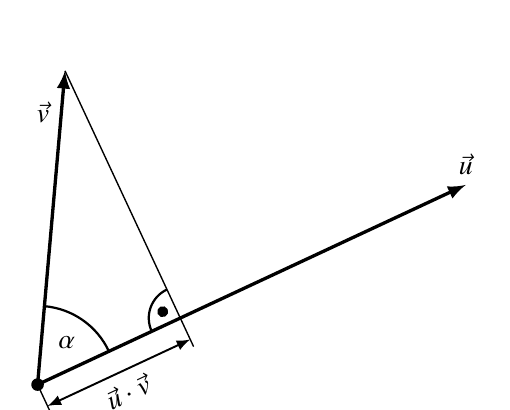
\begin{tikzpicture}[>=latex,thick]

\begin{scope}[rotate=25]

\def\a{60}
\def\l{4}
\def\r{1}

% Vektor u
\draw[->,line width=1.2pt] (0,0)--(6,0);
\node at (6,0) [above] {$\vec{u}$};

% Vektor v
\draw[->,line width=1.2pt] (0,0)--({\l*cos(\a)},{\l*sin(\a)});
\node at ({0.8*\l*cos(\a)},{0.8*\l*sin(\a)}) [above left] {$\vec{v}$};

% Projektion
\draw[line width=0.5pt] ({\l*cos(\a)},{\l*sin(\a)})--({\l*cos(\a)},-0.4);
\draw[line width=0.5pt] (0,0)--(0,-0.4);

% rechter Winkel
\def\rr{0.4}
\draw (2,\rr) arc (90:180:\rr);
\fill ({2-0.42*\rr},{0.42*\rr}) circle[radius=0.07];

% Winkel alpha
\draw (\r,0) arc (0:\a:\r);
\node at ({0.65*\r*cos(\a/2)},{0.65*\r*sin(\a/2)}) {$\alpha$};

% Bemassung
\draw[<->,line width=0.7pt] (0,-0.3)--({\l*cos(\a)},-0.3);
\node at ({0.5*\l*cos(\a)},-0.3) [below,rotate=25] {$\vec{u}\cdot\vec{v}$};

% Nullunkt
\fill (0,0) circle[radius=0.08];

\end{scope}

\end{tikzpicture}

\end{document}


%
% unendlich.tex -- Abschnitt über Dualraum unendlichdimensionaler Vektorräume
%
% (c) 2017 Prof Dr Andreas Müller, Hochschule Rapperswil
%
\section{Dualität und unendlichdimensionale Vektorräume%
\label{section:dualraum:unendlich}}
Für endlichdimensionale Vektorräume haben wir herausgefunden, dass
der Dualraum die gleiche Dimension hat, indem wir zu einer Basis die
duale Basis konstruiert haben.
Ein endlichdimensionaler Vektorraum und sein Dualraum haben daher die
gleiche Dimension.

Für unendlichdimensionale Vektorräume ist die Situation komplizierter.
Wir betrachten dazu einen Vektorraum $V$ mit einer Basis $B$, die jedoch
unendlich viele Elemente enthält.
Um die Situation nicht zu kompliziert werden zu lassen, nehmen wir an,
dass die Basis abzählbar ist, dass heisst dass die Basisvektoren 
numeriert werden können.
Wir schreiben sie
\[
B= \{ b_1,b_2,b_e,\dots\}.
\]
Natürlich können wir weiterhin die Linearformen $b_i^*$ konstruieren.
Das Lemma~\ref{dualraum:lemmaunabh} hat nicht vorausgesetzt, dass der
Vektorraum endlichdimensional muss, daher sind die dualen Linearformen
$b_i^*$ sicher linear unabhängig.

Trotzdem ist die Menge $B^*=\{b_i^*\;|\; i=\mathbb N\}$ keine Basis.
Wir können nämlich eine Linearform $l$ konstruieren, die sich nicht als 
Linearkombination der $b_i^*$ schreiben lässt.
Um den Wert von $l$ auf einem Vektor $v$ festzulegen, schreiben wir
zunächst
\[
v=v_0b_0+v_1b_1+v_2b_2+v_3b_3+\dots,
\]
wobei nur endlich viele der Koeffizienten $v_i$ von $0$ verschieden sind.
Als Wert von $l$ auf $v$ legen wir daher fest
\begin{equation}
l(v) = \sum_{i\in\mathbb N} v_i.
\label{dualraum:linf}
\end{equation}
Da nur endlich viele der $v_i$ von Null verschieden sind, ist die Summe
in \eqref{dualraum:linf} wohldefiniert.
In einem beliebigen Körper $K$ gibt es nämlich im Gegensatz zu den
Körpern $\mathbb R$ und $\mathbb C$ kein Konzept des Grenzwertes und
damit auch keine Möglichkeit, eine unendliche Summe zu berechnen.

Wir müssen jetzt noch einsehen, dass sich $l$ nicht als Linearkombination
von Linearformen $b_i^*$ geschreiben werden kann.
Wir zeigen dies dadurch, dass wir die Annahme, $l$ lasse sich als
Linearkombination der $b_i^*$ schreiben, zu einem Widerspruch führen.
Nehmen wir also an, dass 
\begin{equation}
l=l_0b_0^* + l_1b_1^*+l_2b_2^*+\dots+l_nb_n^*.
\label{dualraum:linf2}
\end{equation}
Wir haben eine endliche Summe geschrieben, weil in einem $K$-Vektorraum
unendliche Summen nicht definiert sind.
Eine Linearkombination kann daher immer nur endlich viele Summanden
enhalten.

Wir werten jetzt $l$ auf dem Basisvektor $b_{n+1}$ aus.
Aus der Definition wissen wir, dass $l(b_{n+1})=1$.
Setzen wir $b_{n+1}$ in die Darstellung 
\eqref{dualraum:linf2} von $l$ ein, erhalten wir
\[
1
=
l(b_{n+1})
=
l_0\underbrace{b_0^*(b_{n+1})}_{\displaystyle=0}
+
l_1\underbrace{b_1^*(b_{n+1})}_{\displaystyle=0}
+
l_2\underbrace{b_2^*(b_{n+1})}_{\displaystyle=0}
+\dots+
l_n\underbrace{b_n^*(b_{n+1})}_{\displaystyle=0}
=
0.
\]
Damit haben wir einen Widerspruch erhalten.
Es ist also nicht möglich, die Linearform $l$ als Linearkombination
von $b_i^*$ zu schreiben.

Dieses Beispiel zeigt, dass der Dualraum eines unendlichdimensionalen
Vektorraumes viele weitere Linearformen enthält, die sich nicht
als Linearkombinationen von $b_i^*$ schreiben lassen.
Man kann sogar zeigen, dass die es überabzählbar viele weitere, linear
unabhängige Linearformen gibt.
Ist nämlich $I\subset\mathbb N$ eine beliebige Teilmenge der natürlichen
Zahlen, dann können wir die Linearform $l_I$ definieren, die auf dem
Vektor $v$ den Wert
\[
l_I(v) = \sum_{i\in I}v_i
\]
haben soll.
Da nur endlich viele der Komponenten $v_i$ von $0$ verschieden sind, 
ist die Summe wohldefiniert.
Die oben beschriebene Linearform $l$ ist nichts anderers als $l_{\mathbb N}$.
Für jede unendliche Teilmenge $I$ ist $l_I$ eine Linearform, die nicht
durch die $b_i^*$ dargestellt werden kann.
Man kann sogar zeigen, dass es unter den $l_I$ überabzählbar viele 
linear unabhängige Linearformen gefunden werden können.
Eine Basis des Dualraumes $V^*$ ist daher viel grösser als eine Basis
von $V$.

Man kann diese Beobachtung auch als Indiz darauf betrachten, dass die
der Begriff des Vektorraumes für unendlichdimensionale Anwendungen noch
etwas zu wenig restriktiv ist.
Tatsächlich zeigt es sich, dass durch Hinzufügen eines Skalarproduktes
und von Grenzwerten eine sehr viel geeignetere Struktur entsteht,
der Hilbert-Raum.
Mehr dazu im Kapitel~\ref{chapter:hilbertspaces}.






%\section{Linearformen}
%Sei $V$ ein Vektorraum über $K$, wobei wir zunächst einschränkend
%annehmen, dass $V$ endlichdimensional ist.
%Für die nachfolgende Diskussion kännen wir uns vorstellen, in $V$ eine Basis
%$(b_i)_{1\le i\le n}$ gewählt zu haben, so dass wir $V$ mit $K^n$
%identifizieren können.
%Ein Vektor in $V$ kann als Spaltenvektor geschrieben werden.
%Die Basisvektoren werden dann mit den Standardbasisvektoren $e_i$
%identifiziert.
%
%Wir versuchen jetzt die Bedeutung der Zeilenvektoren zu ergründen.
%Die Matrizenrechnung lehrt uns, dass wir einen $n$-dimensionalen
%Zeilenvektor $l$ mit einem $n$-dimensionalne Spaltenvektor $v\in K^n$
%nach der Regel
%\[
%l\cdot v
%=
%\begin{pmatrix}
%l_1&l_2&\dots&l_n
%\end{pmatrix}
%\begin{pmatrix}v_1\\v_2\\\vdots\\v_n\end{pmatrix}
%=
%l_1v_1+l_2v_2+\dots+l_nv_n
%\]
%multiplizieren können.
%Linearformen in einem $n$-dimensionalen Raum können also selbst
%als den $n$-dimensionalen Vektorraum Zeilenvektoren der Länge $n$
%betrachtet werden.
%
%Dass die Linearformen selbst einen Vektorraum bilden, wussten wir
%natürlich schon länger.
%In Kapitel~\ref{chapter:vektorraum} haben wir bereits gezeigt,
%dass die Menge lineare Abbildungen ein Vektorraum ist.
%Da $K$ selbst auch ein eindimensionaler Vektorraum ist, ist
%$V^*=\operatorname{Hom}(V,K)$ ebenfalls ein Vektorraum, er heisst
%der {\em Dualraum}.
%\index{Dualraum}%
%
%Seien jetzt $U,V$ zwei $K$-Vektorräume und $f\colon U\to V$ eine lineare
%Abbildung zwischen den beiden Vektorräumen.
%Aus $f$ können wir eine lineare Abbildung zwischen den Dulräumen
%$U^*$ und $V^*$ wie folgt konstruieren.
%Ist $l\in V^*$ eine Linearform, dann ist die Abbildung
%\[
%f^*(l)\colon U\to K:u\mapsto f^*(l)(u)=l(f(u)) = l\circ f(u)
%\]
%linear, also eine Linearform in $U^*$.
%Die Abbildung $f^*$ ist also eine lineare Abbildung $f^*\colon V^*\to U^*$
%zwischen den Dualräumen.
%
%Es wird etwas klarer, was hier vorgeht, wenn wir die Konstruktion
%des Dualraum etwas umständlicher als $\operatorname{Dual}(U)=U^*$
%schreiben.
%Die von $f$ induzierte Abbildung der Dualräume wird dann mit
%\[
%f^*
%=
%\operatorname{Dual}(f)
%\colon 
%\operatorname{Dual}(V)
%\to
%\operatorname{Dual}(U)
%\]
%bezeichnet.
%In der Terminologie von Kapitel~\ref{chapter:kategorien} ist
%$\operatorname{Dual}$ ein kontravarianter Funktor in der Kategorie
%der $K$-Vektorräume.
%
%\section{Dualbasis}
%Bei endlichdimensionalen Vektorräumen konnten wir mit Hilfe einer Basis
%die abstrakte Struktur des Vektorraumes auf die viel einfachere und
%übersichtlichere Situation der $n$-dimensionalen Spaltenvektoren 
%reduzieren.
%Wir sind also bestrebt, aus einer Basis des Vektorraums eine passende
%Basis des Dualraumes zu konstruieren, und damit auch den
%Dualraum auf einen Raum von Spaltenvektoren zu reduzieren.
%
%Sei daher jetzt $V$ ein $K$-Vektorraum und $B$ eine Basis von $V$.
%Wir suchen eine Basis des Dualraumes $V^*$.
%Da sich jeder Vektor in $V$ als Linearkombination von Basisvektoren
%schreiben lässt, ist eine Linearform in $V^*$ festgelegt durch die Werte
%auf den Basisvektoren.
%Wir konstruieren daher zu jedem Vektor $b\in B$ die {\em duale Linearform}
%mittels der Definition
%\begin{equation}
%b^*\colon V\to K:b'\mapsto
%\begin{cases}
%1&\qquad b'=b\\
%0&\qquad b'\ne b,\; b'\in B
%\end{cases}
%\label{dualraum:dualeform}
%\end{equation}
%Die duale Linearform $b^*$ hat also den Wert $1$ auf dem Basisvektor $b$
%und den Wert $0$ auf allen anderen Basisvektoren.
%Ist $v=v_1b_1+\dots+v_nb_n$, dann ist
%$b_i^*(v)=v_i$, d.~h.~die dualen Lineareformen der Basisvektoren können
%dazu verwendet werden, die Komponenten eines Vektors in der Basis $B$
%zu berechnen.
%
%Sei jetzt zusätzlich $V$ ein $n$-dimensionaler Vektorraum sein mit
%der Basis $B=\{b_1,\dots,b_n\}$.
%Vektoren in $V$ können dann als Linearkombinationen 
%\[
%v=v_1b_1+\dots+v_nb_n
%\]
%von Basisvektoren schreiben.
%Die zu $b_i$ duale Linearform $b_i^*$ hat auf $v$ den Wert
%\[
%b_i^*(v)
%=
%v_1\underbrace{b_i^*(b_1)}_{\displaystyle=0}
%+
%\dots
%+
%v_i\underbrace{b_i^*(b_i)}_{\displaystyle=1}
%+
%\dots
%+
%v_n\underbrace{b_i^*(b_n)}_{\displaystyle=0}
%=
%v_i
%\]
%Sei weiter $l$ eine Linearform auf $V$.
%Wir wollen $l$ als Linearkombination von dualen Linearformen $b^*$
%mit $b\in B$ schreiben.
%Wir suchen also Zahlen $l_1,\dots,l_n$ derart, dass
%\[
%l = l_1b_1^* + \dots + l_nb_n^*.
%\]
%Durch Einsetzen der Basisvektoren folgt
%\[
%l(b_i)
%=
%l_1b_1^*(b_i) + \dots + l_nb_n^*(b_i)
%=
%l_i,
%\]
%damit habe wir die $l_i$ bereits gefunden.
%Damit ist nachgewiesen, dass die $b_i^*$ den Dualraum $V^*$ erzeugt.
%
%Wir möchten jetzt auch noch zeigen, dass die dualen Linearformen linear
%unabhängig sind.
%Wir formulieren dies wieder etwas abstrakter und geben einen formalen
%Beweis.
%
%\begin{lemma}
%\label{dualraum:lemmaunabh}
%Sie $V$ ein $K$-Vektorraum mit Basis $B$, dann ist die
%Menge der dualen Linearformen $B^* = \{b^*\;|\;b\in B\}$ linear
%unabhängig im $K$-Vektorraum $V^*$.
%\end{lemma}
%
%\begin{proof}[Beweis]
%Wir müssen zeigen, dass eine verschwindende Linearkombination 
%\[
%l
%=
%\lambda_1 b_1^* + \dots +\lambda_n b_n^* = 0
%\]
%nur für $\lambda_1=\dots=\lambda_n=0$ möglich ist.
%Dazu wenden wir $l$ auf die Basisvektoren $b_i$ an und erhalten
%\[
%0
%=
%l(b_i)
%=
%\lambda_1b_1^*(b_i) + \dots + \lambda_nb_n^*(b_i)
%=
%\lambda_i.
%\]
%Damit haben wir nachgerechnet, dass $\lambda_i=0$ gilt, die einzige
%verschwindende Linearkombiantion von Basisformen $b^*\in B^*$ ist
%daher die Nullform.
%\end{proof}
%
%Damit haben wir insgesamt den folgenden Satz bewiesen.
%
%\begin{satz}
%Ist $V$ ein $n$-dimensionaler $K$-Vektorraum mit Basis $B=\{b_1,\dots,b_n\}$,
%dann ist $V^*$ ein $n$-dimensionaler $K$-Vektorraum mit 
%Basis $B^*=\{b_1^*,\dots,b_n^*\}$.
%\end{satz}
%
%Die Basis $B^*$ von $V^*$ heisst die Dualbasis.
%In den folgenden Abschnitten betrachten wir nur endlichdimensionale
%Vektorräume und ihre Dualräume, die ebenfalls endlichdimensional sind,
%und kehren erst in
%Abschnitt~\ref{section:dualraum:unendlich} zu den unendlichdimensionalen
%und der speziellen Struktur ihrer Dualräume zurück.
%
%\section{Transposition -- das oberflächliche Markenzeichen der Dualität%
%\label{dualraum:section:transposition}}
%Einen $n$-dimensionalen Vektorraum $V$ können wir mit Hilfe einer
%Basis immer sofort in den Vektorraum der $n$-dimensionalen
%Spaltenvektoren $K^n$ umwandeln.
%Als Basisvektoren können wir die Standardbasisvektoren $e_i$ verwenden,
%die genau in Zeile $i$ eine $1$ haben und sonst überall $0$.
%
%In Abschnitt~\ref{section:vektorraum:linabb} wurde gezeigt, wie zu
%einer linearen Abbildung eine Matrix gehört.
%Im Falle einer Linearform ist der Bildraum eindimensional, sie muss
%also als $1\times n$-Matrix dargestellt werden können.
%Es stellt sich daher die Frage, welche $1\times n$-Matrizen die
%dualen Linearformen $e_i^*$ darstellen.
%
%Nach Definition \eqref{dualraum:dualeform} der dualen Linearform
%muss gelten
%\[
%e_i^* e_j
%=
%\delta_{ij}
%=
%\begin{cases}
%1&\qquad i=j\\
%0&\qquad \text{sonst.}
%\end{cases}
%\]
%Dies ist nur möglich, wenn $e_i^*$ die Matrix
%\[
%e_i^*
%=
%\begin{pmatrix}
%0&\dots&1&\dots&0
%\end{pmatrix}
%\]
%mit einer $1$ an der $i$-ten Stelle und $0$ sonst.
%Man kann also schreiben $e_i^*=e_i^t$.
%
%Wir betrachten jetzt eine lineare Abbildung $f\colon U=K^n\to V=K^m$.
%Aus Abschnitt~\ref{section:vektorraum:linabb} ist bekannt, dass
%$f$ durch eine $m\times n$-Matrix $A$ beschreiben werden kann:
%\[
%\begin{pmatrix}
%v_1\\\vdots\\v_m
%\end{pmatrix}
%=
%\begin{pmatrix}
%a_{11}&\dots &a_{1n}\\
%\vdots&\ddots&\vdots\\
%a_{m1}&\dots &a_{mn}
%\end{pmatrix}
%\begin{pmatrix}
%u_1\\\vdots\\u_n
%\end{pmatrix}.
%\]
%Aus einer Linearform $l$ in $V^*$ mit der Matrix
%\[
%\begin{pmatrix}l_1&\dots&l_n\end{pmatrix}
%\]
%wird durch Anwendung von $f^*$ die Linearform $f^*(l)=l\circ f$, wir
%wollen die Matrix von $f^*(l)$ ermitteln.
%Dazu genügt es, die Werte von $f^*(l)$ auf einem Vektor $u\in K^n$
%zu bestimmen.
%Wir berechnen also
%\[
%f^*(l)(u)
%=
%l(f(u))
%=
%\begin{pmatrix}l_1&\dots&l_n\end{pmatrix}
%\begin{pmatrix}
%a_{11}&\dots &a_{1n}\\
%\vdots&\ddots&\vdots\\
%a_{m1}&\dots &a_{mn}
%\end{pmatrix}
%\begin{pmatrix}
%u_1\\\vdots\\u_n
%\end{pmatrix}
%=
%\sum_{j=1}^nl_j \sum_{i=1}^m a_{ji}u_i
%=
%\sum_{i=1}^m
%\biggl(
%\sum_{j=1}^nl_j a_{ji}
%\biggr)
%u_i.
%\]
%Die Linearform $f^*(l)$ hat daher die $1\times m$-Matrix
%\begin{equation}
%\begin{pmatrix}
%\sum_{j=1}^nl_j a_{j1}
%&\dots&
%\sum_{j=1}^nl_j a_{jm}
%\end{pmatrix}
%=
%lA.
%\label{dualraum:transp}
%\end{equation}
%Die duale Abbildung $f^*$ wird also durch Rechtsmultiplikation der
%Zeilenvektoren mit $A$ vermittelt.
%
%Verwendet man die duale Basis dazu, den Dualraum $V^*$ von $V$
%mit Spaltenvektoren $K^n$ zu identifizieren dann ist der 
%zu $l$ gehörende Spaltenvektor $l^t$.
%Die duale Abbildung $f^*\colon V^*\to U^*$ kann mit Hilfe der
%Dualbasis ebenfalls als $n\times m$-Matrix beschrieben werden.
%Aus \eqref{dualraum:transp} kann man ablesen, dass diese Matrix
%$A^t$ sein muss.
%Die Transposition ist also nichts anderes als ein Ausdruck des Übergangs
%zu einer Darstellung in der dualen Basis.
%
%\section{Dualität und Skalarprodukt}
%In der elementaren Vektorgeometrie verwendet man als Skalarprodukt
%zweier $n$-dimensionaler Spaltenvektoren $u,v\in K^n$ die Grösse
%\[
%u\cdot v
%=
%u^t v
%=
%u_1v_1+\dots+u_nv_n.
%\]
%Im Lichte der Betrachtungen von Abschnitt~\ref{dualraum:section:transposition}
%erzeugt die Transposition zu jedem Vektor $u\in K^n$ eine Linearform
%$u^t\in K^{n*}$.
%Jede Linearform ensteht durch Transposition aus einem Vektor.
%Das Skalarprodukt in einem endlichdimensionalen Vektorraum kann 
%daher verstanden werden als der Ausdruck der Tatsache, dass die
%Transposition den Vektorraum mit seinem Dualraum identifizieren kann.
%
%In Abschnitt~\ref{section:dualraum:unendlich} wird gezeigt, dass
%eine solche Identifikation bei unendlichdimensionalen Vektorräumen
%nicht mehr möglich ist.
%Unendlichdimensionale Vektorräume haben einen sehr viel grösseren Dualraum.
%
%Um diesen Unterschied zwischen Skalarprodukt und Auswertung von Linearformen
%deutlicher zu machen, lohnt es sich, eine Notation zu verwenden, welche
%die Gemeinsamkeiten und Unterschiede deutlicher macht.
%Für einen Vektor $u\in V$ und eine Linearform $v\in  V^*$ schreiben
%wir für die Auswertung der Linearform $v$ auf $u$
%\[
%\langle v,u\rangle = v(u).
%\]
%Für das Skalarprodukt zweier Vektoren $v$ und $u$ in $V$  schreiben wir
%\[
%(v,u) = u\cdot v.
%\]
%Damit kann man für $v,u\in K^n$ schreiben
%\[
%\langle v^t,u\rangle = (v,u),
%\]
%bzw.~für $v\in K^{n*}$ und $u\in K^n$
%\[
%\langle v, u\rangle
%=
%(v^t,u).
%\]
%In dieser Form wird es in Kapitel~\ref{chapter:hilbertspaces}
%möglich sein, den Übergang zwischen Dualraum
%und Skalarprodukt auch in einem geeignet angereicherten,
%unendlichdimensionalen Vektorraum
%zu ermöglichen, selbst wenn die Darstellung der Vektoren als
%Spaltenvektoren nicht möglich ist.
%
%\section{Dualität und unendlichdimensionale Vektorräume%
%\label{section:dualraum:unendlich}}
%Für endlichdimensionale Vektorräume haben wir herausgefunden, dass
%der Dualraum die gleiche Dimension hat, indem wir zu einer Basis die
%duale Basis konstruiert haben.
%Ein endlichdimensionaler Vektorraum und sein Dualraum haben daher die
%gleiche Dimension.
%
%Für unendlichdimensionale Vektorräume ist die Situation komplizierter.
%Wir betrachten dazu einen Vektorraum $V$ mit einer Basis $B$, die jedoch
%unendlich viele Elemente enthält.
%Um die Situation nicht zu kompliziert werden zu lassen, nehmen wir an,
%dass die Basis abzählbar ist, dass heisst dass die Basisvektoren 
%numeriert werden können.
%Wir schreiben sie
%\[
%B= \{ b_1,b_2,b_e,\dots\}.
%\]
%Natürlich können wir weiterhin die Linearformen $b_i^*$ konstruieren.
%Das Lemma~\ref{dualraum:lemmaunabh} hat nicht vorausgesetzt, dass der
%Vektorraum endlichdimensional muss, daher sind die dualen Linearformen
%$b_i^*$ sicher linear unabhängig.
%
%Trotzdem ist die Menge $B^*=\{b_i^*\;|\; i=\mathbb N\}$ keine Basis.
%Wir können nämlich eine Linearform $l$ konstruieren, die sich nicht als 
%Linearkombination der $b_i^*$ schreiben lässt.
%Um den Wert von $l$ auf einem Vektor $v$ festzulegen, schreiben wir
%zunächst
%\[
%v=v_0b_0+v_1b_1+v_2b_2+v_3b_3+\dots,
%\]
%wobei nur endlich viele der Koeffizienten $v_i$ von $0$ verschieden sind.
%Als Wert von $l$ auf $v$ legen wir daher fest
%\begin{equation}
%l(v) = \sum_{i\in\mathbb N} v_i.
%\label{dualraum:linf}
%\end{equation}
%Da nur endlich viele der $v_i$ von Null verschieden sind, ist die Summe
%in \eqref{dualraum:linf} wohldefiniert.
%In einem beliebigen Körper $K$ gibt es nämlich im Gegensatz zu den
%Körpern $\mathbb R$ und $\mathbb C$ kein Konzept des Grenzwertes und
%damit auch keine Möglichkeit, eine unendliche Summe zu berechnen.
%
%Wir müssen jetzt noch einsehen, dass sich $l$ nicht als Linearkombination
%von Linearformen $b_i^*$ geschreiben werden kann.
%Wir zeigen dies dadurch, dass wir die Annahme, $l$ lasse sich als
%Linearkombination der $b_i^*$ schreiben, zu einem Widerspruch führen.
%Nehmen wir also an, dass 
%\begin{equation}
%l=l_0b_0^* + l_1b_1^*+l_2b_2^*+\dots+l_nb_n^*.
%\label{dualraum:linf2}
%\end{equation}
%Wir haben eine endliche Summe geschrieben, weil in einem $K$-Vektorraum
%unendliche Summen nicht definiert sind.
%Eine Linearkombination kann daher immer nur endlich viele Summanden
%enhalten.
%
%Wir werten jetzt $l$ auf dem Basisvektor $b_{n+1}$ aus.
%Aus der Definition wissen wir, dass $l(b_{n+1})=1$.
%Setzen wir $b_{n+1}$ in die Darstellung 
%\eqref{dualraum:linf2} von $l$ ein, erhalten wir
%\[
%1
%=
%l(b_{n+1})
%=
%l_0\underbrace{b_0^*(b_{n+1})}_{\displaystyle=0}
%+
%l_1\underbrace{b_1^*(b_{n+1})}_{\displaystyle=0}
%+
%l_2\underbrace{b_2^*(b_{n+1})}_{\displaystyle=0}
%+\dots+
%l_n\underbrace{b_n^*(b_{n+1})}_{\displaystyle=0}
%=
%0.
%\]
%Damit haben wir einen Widerspruch erhalten.
%Es ist also nicht möglich, die Linearform $l$ als Linearkombination
%von $b_i^*$ zu schreiben.
%
%Dieses Beispiel zeigt, dass der Dualraum eines unendlichdimensionalen
%Vektorraumes viele weitere Linearformen enthält, die sich nicht
%als Linearkombinationen von $b_i^*$ schreiben lassen.
%Man kann sogar zeigen, dass die es überabzählbar viele weitere, linear
%unabhängige Linearformen gibt.
%Ist nämlich $I\subset\mathbb N$ eine beliebige Teilmenge der natürlichen
%Zahlen, dann können wir die Linearform $l_I$ definieren, die auf dem
%Vektor $v$ den Wert
%\[
%l_I(v) = \sum_{i\in I}v_i
%\]
%haben soll.
%Da nur endlich viele der Komponenten $v_i$ von $0$ verschieden sind, 
%ist die Summe wohldefiniert.
%Die oben beschriebene Linearform $l$ ist nichts anderers als $l_{\mathbb N}$.
%Für jede unendliche Teilmenge $I$ ist $l_I$ eine Linearform, die nicht
%durch die $b_i^*$ dargestellt werden kann.
%Man kann sogar zeigen, dass es unter den $l_I$ überabzählbar viele 
%linear unabhängige Linearformen gefunden werden können.
%Eine Basis des Dualraumes $V^*$ ist daher viel grösser als eine Basis
%von $V$.
%
%Man kann diese Beobachtung auch als Indiz darauf betrachten, dass die
%der Begriff des Vektorraumes für unendlichdimensionale Anwendungen noch
%etwas zu wenig restriktiv ist.
%Tatsächlich zeigt es sich, dass durch Hinzufügen eines Skalarproduktes
%und von Grenzwerten eine sehr viel geeignetere Struktur entsteht,
%der Hilbert-Raum.
%Mehr dazu im Kapitel~\ref{chapter:hilbertspaces}.
%
%
%
%

%
% tensor.tex -- Tensoralgebra (Indexgymnastik)
%
% (c) 2017 Prof Dr Andreas Müller, Hochschule Rapperswil
%
\chapter{Tensoren}
\rhead{Tensoren}
Matrizen und Vektoren sind ein- und zweidimensionale Anordnungen von
Zahlen.
Matrizen operieren linear auf Vektoren und erzeugen neue Vektoren.
Kann dieses Konzept verallgemeinert werden auf Operationen, die
auf mehreren Vektoren oder sogar Matrizen wirken?
Tensoren beantworten diese Frage.


\section{Vektor, Matrix, Tensor}
\subsection{Operationen --- Summationskonvention}
\subsection{Tensoren beliebiger Stufe}
\subsection{Symmetrische und Antisymmetrische Tensoren}
\subsection{Skalarprodukt und Metrik}

\section{Kovarianz und Kontravarianz}
\subsection{Basistransformation}
\subsection{Kovarianz und Kontravarianz}

\section{Anwendungen}
\subsection{Tangentialvektoren einer Mannigfaltigkeit}
\subsection{Metrik auf einer Mannigfaltigkeit}
\subsection{Kovariante Ableitung, Geodäten und Krümmung}
\subsection{Symbol eines Differentialoperators als Tensor}


%
% hilbertraum.tex -- Theorie der Hilberträume
%
% (c) 2017 Prof Dr Andreas Müller, Hochschule Rapperswil
%
\chapter{Hilberträume
\label{chapter:hilbertspaces}}
\lhead{Hilberraum}
\rhead{}
Die Theorie der Vektorräume mit einem Skalarprodukt wird im Unterricht
üblicherweise nur am Beispiel des Vektorraums $\mathbb R^n$ dargestellt.
Dabei werden die Studierenden kurze Zeit später mit der Theorie
der Fourier-Reihen konfrontiert, die in natürlicher Weise in einem
unendlichdimensionalen Vektorraum mit einem Skalarprodukt situiert ist.

\section{Skalarprodukt und Norm}
\rhead{Skalarprodukt und Norm}
Da die Theorie eines Vektorraumes mit Skalarprodukt formuliert werden
soll unabhängig von der konkreten Darstellung der Vektoren als 
Spaltenvektoren, muss das Skalaprodukt ebenfalls unabhängig von einer
solchen Darstellung definiert werden.
Die axiomatische Methode bietet sich hierfür an.

\begin{definition}
\label{hilbert:hermitescheform}
Sei $V$ ein komplexer Vektorraum.
Eine Funktion $\langle\;,\;\rangle\colon V\times V\to\mathbb C$ heisst
{\em hermitesch}, wenn sie folgende Eigenschaften hat
\begin{enumerate}[label={\bf HF.\arabic*},itemsep=0mm]
\item $\langle\;,\;\rangle$ ist linear im ersten und konjugiert-linear
im zweiten Argument:
\begin{align*}
\langle x+x',y\rangle &=\langle x,y\rangle + \langle x',y\rangle
&
\langle x,y+y'\rangle &=\langle x,y\rangle + \langle x,y'\rangle
\\
\langle\lambda x,y\rangle&=\lambda\langle x,y\rangle
&
\langle x,\lambda y\rangle&=\overline\lambda\langle x,y\rangle
\end{align*}
für alle $x,x',y,y'\in V$.
\item Für alle $x,y\in V$ gilt
$\langle x,y\rangle=\overline{\langle y,x\rangle}$.
\end{enumerate}
\end{definition}
Eine hermitsche Form ist noch nicht geeignet, die Rolle eines
Skalarproduktes zu übernehmen, denn wir möchten ja $\langle x,x\rangle$
als Quadrat der Länge eines Vektors $x$ interpretieren.
Dazu muss zunächst mal sichergestellt sein, dass $\langle x,x\rangle$
eine reelle Zahl ist.
Doch dies folgt aus Axiom (HF.2) einer hermiteschen Form.
Vertauscht man die beiden Argument in $\langle x,x\rangle$, ändert
sich natürlich nichts, und daher folgt
\[
\langle x,x\rangle = \overline{\langle x,x\rangle}
\qquad\Rightarrow\qquad
\langle x,x\rangle\in\mathbb R.
\]

Damit $\langle x,x\rangle$ das Quadrat der Länge sein kann, darf
$\langle x,x\rangle$ nicht negativ wird, was
durch die Axiome nicht sichergestellt wird.
Ist nämlich $\langle\;,\;\rangle$ eine hermitesche Form, dann ist
auch $-\langle\;,\;\rangle$ eine hermitesche Form.
Die Definition muss daher verfeinert werden:

\begin{definition}
\label{hilbert:postiveform}
Eine hermitesche Form heisst {\em positiv}, wenn gilt
$\langle x,x\rangle \ge 0$ für alle $x\in V$.
\end{definition}

Positive hermitesche Formen haben bereits eine wichtige Eigenschaft,
die für die Definition der Länge erforderlich.

\begin{satz} Ist $\langle\;,\;\rangle$ eine positive hermitesche
Form, dann gilt die Cauchy-Schwarz-Ungleichung
\[
|\langle x,y\rangle|^2 \le \langle x,x\rangle\langle y,y\rangle
\]
für beliebige Vektoren $x,y\in V$.
\end{satz}

\begin{proof}[Beweis]
Wir betrachten den Vektor $x+\lambda y$.
Da $\langle\;,\;\rangle$ positiv ist, gilt 
$\langle x+\lambda y,x+\lambda y\rangle \ge 0$.
Mit der Linearität von $\langle\;,\;\rangle$ können wir dies
aber auch ausrechnen:
\begin{align*}
0&\le
\langle x+\lambda y,x+\lambda y\rangle
\\
&=
\langle x,x\rangle
+
\langle \lambda y,x\rangle
+
\langle x,\lambda y\rangle
+
\langle \lambda y,\lambda y\rangle
\\
&=
\langle x,x\rangle
+
\lambda\langle y,x\rangle
+
\overline{\lambda}\langle x,y\rangle
+
\lambda\overline{\lambda}\langle y,y\rangle
\\
&=
\langle x,x\rangle
+
\lambda\langle y,x\rangle
+
\overline{\lambda}\langle y,x\rangle
+
|\lambda|^2\langle y,y\rangle
\end{align*}
Falls $\langle y,y\rangle >0$
setzt man $\lambda = - \langle x,y\rangle/\langle y,y\rangle$.
Dann folgt
\begin{align*}
0
&\le
\langle x,x\rangle
-
2\frac{\langle x,y\rangle}{\langle y,y\rangle}\langle y,x\rangle
+
\frac{|\langle y,x\rangle|^2}{\langle y,y\rangle^2}\langle y,y\rangle
\\
&=
\langle x,x\rangle
-2
\frac{|\langle x,y\rangle|^2}{\langle y,y\rangle}
+
\frac{|\langle y,x\rangle|^2}{\langle y,y\rangle^2}\langle y,y\rangle
\\
&=
\langle x,x\rangle
-
\frac{|\langle x,y\rangle|^2}{\langle y,y\rangle}.
\end{align*}
Durch Multiplizieren mit $\langle y,y\rangle$ erhält man daraus
\begin{align*}
0&\le
\langle x,x\rangle\langle y,y\rangle
-
|\langle x,y\rangle|^2
\\
\Rightarrow\qquad
|\langle x,y\rangle|^2
&\le
\langle x,x\rangle\langle y,y\rangle.
\end{align*}

"Ahnlich kann vorgegangen werden, wenn $\langle x,x\rangle > 0$ ist und
$\langle y,y\rangle =0$.

Im Fall $\langle x,x\rangle=\langle y,y\rangle=0$ verwendet man 
$\lambda = -\langle x,y\rangle$ und erhält
\begin{align*}
0
&\le
\langle x,x\rangle
+
\lambda\langle y,x\rangle
+
\overline{\lambda}\langle y,x\rangle
+
|\lambda|^2\langle y,y\rangle
\\
&=
-\langle x,y\rangle\langle y,x\rangle
-\langle y,x\rangle\langle x,y\rangle
=
-2|\langle x,y\rangle|^2
\\
\Rightarrow\qquad
2|\langle x,y\rangle|^2
&\le 0.
\end{align*}
Daraus folgt $\langle x,y\rangle = 0$, ein Spezialfall der
Cauchy-Schwarz-Ungleichung.
\end{proof}

Auch mit dieser Definition ist es immer noch möglich, dass Vektoren,
die von $0$ verschieden sind, Skalarprodukt $0$ haben.
Dies verhindert die folgend Erweiterung der Definition

\begin{definition}
\label{hilbert:postivdefiniteform}
Eine hermitesche Form $\langle\;,\;\rangle$ heisst {\em positiv definit},
wenn $\langle x,x\rangle > 0$ für alle Vektoren $x\ne 0$ in $V$.
\end{definition}

Eine positiv definite hermitesche Form erlaubt nun die Norm
eines Vektors zu definieren

\begin{definition}
Ist $\langle \;,\;\rangle$ eine positiv definite hermitesche Form
auf $V$, dann heisst $\|x\| = \sqrt{\langle x,x\rangle}$ die {\em Norm}
des Vektors $x\in V$.
\end{definition}

Diese Norm erfüllt die Dreiecksungleichung, wie man mit folgender
Rechnung einsehen kann:
\begin{align*}
\|x+y\|^2
&=
\langle x+y,x+y\rangle
\\
&=
\langle x,x\rangle
+
\langle x,y\rangle
+
\langle y,x\rangle
+
\langle y,y\rangle
\\
&=
\|x\|^2 + \|y\|^2
+ 2\operatorname{Re}\langle x,y\rangle
\\
&\le
\|x\|^2 + 2\|x\|\cdot \|y\| + \|y\|^2 = (\|x\| + \|y\|)^2
\\
\Rightarrow\qquad
\|x+y\|
&\le
\|x\| + \|y\|
\end{align*}
Damit ist die Dreiecksungleichung bewiesen.

\begin{definition}
Ein (komplexer) Prähilbertraum ist ein komplexer Vektorraum mit
einer positiv definiten hermiteschen Form $\langle\;,\;\rangle$
auch genannt das {\em Skalarprodukt} des Prähilbertraumes.
\end{definition}

\section{Hilbertraum}
\rhead{Hilbertraum}
Die rationalen komplexen Zahlen $\mathbb Q(i)=\{a+bi\,|\,a,b\in\mathbb Q\}$
können als komplexer Hilbertraum mit dem Skalarprodukt
$\langle x,y\rangle = \overline{x}y$ betrachtet werden.
Die Norm von $x=a+bi$ ist $\|x\|^2=a^2+b^2$.
Auf den rationalen Zahlen ist die Norm genau der Betrag, Cauchy-Folgen
in $\mathbb Q$ sind also automatisch auch Cauchy-Folgen im
Prähilbertraum $\mathbb Q(i)$.
Es ist aber auch wohlbekannt dass, eine Cauchy-Folge in $\mathbb Q$
nicht konvergent sein muss.

Wir möchten den Begriff des Hilbertraums als die natürlich Bühne zum
Beispiel für die Fourier-Theorie etablieren, in der das Summieren von
Reihen wie einer Fourier-Reihe
\[
f(x) = \frac{a_0}2+\sum_{k=1}^\infty (a_k\cos kx+b_k\sin kx)
\]
wohldefiniert sein soll.
Wir müssen daher fordern, dass Cauchy-Folgen einen Grenzwert haben,
und definieren daher eine Hilbertraum wie folgt.

\begin{definition}
Ein Prähilbertraum $H$ heisst ein {\em Hilbertraum}, wenn jede er 
vollständig ist, d.~h.~wenn jede Cauchy-Folge einen Grenzwert in $H$ hat.
\end{definition}

\begin{beispiel}[Endlichdimensionale komplexe Vektorräume]
Der Vektorraum $\mathbb C^n$ ist in natürlicher Weise ein Prähilbertraum
mit dem Skalarprodukt $\langle u,v\rangle = \overline{u}^t v$.
Da $\mathbb C$ vollständig ist, ist $\mathbb C^n$ aber auch ein
Hilbertraum.
\end{beispiel}

\begin{beispiel}[Periodische Funktionen]
Sei $C(S^1, \mathbb C)$ die Menge der stetigen, komplexwertigen Funktionen 
von $S^1 = \mathbb R/2\pi\mathbb Z$.
Das Skalarprodukt
\[
\langle f,g\rangle = \frac1{\sqrt{2\pi}}\int_0^{2\pi} \overline{f(x)} g(x)\,dx
\]
macht $C(S^1,\mathbb C)$ zu einem Prähilbertraum.
Er kann aber kein Hilbertraum sein, denn die Funktionenfolge
\[
f_n(x)=\root{2n+1}\of{\sin x},\qquad n\in\mathbb N
\]
konvergiert gegen die Rechteckfunktion
\[
f(x)=\begin{cases}
1&\qquad 0<x<\pi\\
-1&\qquad \pi<x<2\pi\\
0&\qquad\text{sonst}
\end{cases}
\]
Diese Funktion ist nicht stetig, also nicht in $C(S^1,\mathbb C)$, es existiert
also zwar ein Grenzwert, aber er liegt nicht im Raum $H$ drin.
\end{beispiel}

\begin{beispiel}[Der Hilbertraum $l^2$]
Betrachte den Vektorraum $l^2$ der Folgen komplexer Zahlen
$(a_n)_{n\in\mathbb N}$ so, dass 
\[
\sum_{n=0}^\infty |a_n|^2 <\infty.
\]
Wir definieren das Skalarprodukt von zwei Folgen $a,b\in l^2$ als
\[
\langle a,b\rangle
=
\sum_{n=0}^\infty a_n \overline b_n.
\]
Diese Skalarprodukt ist tatsächlich eine hermitesche Form:
\begin{align*}
\langle \lambda a,b\rangle
&=
\sum_{n=0}^\infty \overline{\lambda a_n} b_n
=
\overline\lambda\sum_{n=0}^\infty \overline a_nb_n
=
\overline\lambda \langle a,b\rangle
\\
\langle a,\lambda b\rangle
&=
\sum_{n=0}^\infty \overline{a_n} \lambda b_n
=
\lambda\sum_{n=0}^\infty \overline a_nb_n
=
\lambda \langle a,b\rangle
\\
\langle a+b,c\rangle
&=
\sum_{n=0}^\infty (\overline{a_n+b_n})c_n
=
\sum_{n=0}^\infty \overline a_n c_n + \sum_{n=0}^\infty \overline b_n c_n
=
\langle a,c\rangle + \langle b,c\rangle
\end{align*}
Um zu zeigen, dass $l^2$ ein Hilbertraum ist, müssen wir zeigen, dass 
Cauchy-Folgen in $l^2$ konvergieren.
Sei also $a^(k)$  eine Cauchy-Folge von Vektoren in $l^2$.
Es folgt, dass auch jede Komponente $a^{(k)}_n$ eine Cauchy-Folge in
$\mathbb C$ ist, und damit konvergent.
Insbesondere ist die Folge
\[
a_n = \lim_{k\to\infty} a_n^{(k)}
\]
der Kandidat für den Grenzwert der Folge von $a^{(k)}$.
Wir müssen zunächst zeigen, dass $a\in l^2$, dass also die
Komponenten von $a$ quadratsummierbar sind.

TODO
\end{beispiel}

\section{Orthonormalbasis}
\rhead{Orthonormalbasis}
In einem endlich dimensionalen Vektorraum kann immer eine Basis aus
orthonormierten Vektoren gefunden werden.
In einem Hilbertraum ist Orthogonalität dank des Skalarproduktes definierbar,
und damit stellt sich die Frage, ob es auch in einem Hilbert-Raum
immer eine Orthonormalbasis gibt.

\begin{proposition}
\label{supplement:hilbertraum:orthogonalkomplement}
Sei $H$ ein Hilbertraum und $V\subset H$ ein Unterraum.
Dann ist
\[
V^\perp = \{u\in H\,|\, \langle u,v\rangle=0\forall v\in V\}
\]
ein Hilbertraum.
\end{proposition}

\begin{proof}[Beweis]
Zunächst ist klar, dass $V^\perp$ ein Prähilbertraum ist, es muss
also nur noch gezeigt werden, dass $V^\perp$ vollständig ist.
Sei also $x_n\in V^\perp$ eine Cauchy-Folge.
Weil $H$ ein Vektorraum ist, gibt es einen Grenzwert $x\in H$, mit
\[
\lim_{n\to\infty} x_n=x.
\]
Es ist zu zeigen, dass $x\in V^\perp$.
Für jedes $v\in V$ ist die Abbildung $u\mapsto \langle u,v\rangle$ eine
stetige Abbildung, daher gilt
\[
0=\lim_{n\to\infty} \langle x_n,v\rangle = \langle x,v\rangle,
\]
für alle $v\in V$.
Es folgt $x\in V^\perp$, womit die Proposition bewiesen ist.
\end{proof}

\begin{proposition}
Sie $V\subset H$ ein Unterraum des Hilbertraumes $H$, dann ist
$(V^\perp)^\perp=\overline V$.
\end{proposition}

\begin{proof}[Beweis]
Aus Proposition~\ref{supplement:hilbertraum:orthogonalkomplement}
schliessen wir, dass $(V^\perp)^\perp)$ ein Hilbertraum und damit
abgeschlossen ist.
Ausserdem ist
\[
v\in V
\quad\Rightarrow\quad
\langle v,u\rangle = 0\forall u\in V^\perp
\quad\Rightarrow\quad
v\in (V^\perp)^\perp,
\]
also ist $V\subset (V^\perp)^\perp$.
Insbesondere schliessen wir, dass $\overline V\subset (V^\perp)^\perp$.

TODO
\end{proof}

\section{Operatoren auf einem Hilbert-Raum}
\rhead{Operatoren auf einem Hilbert-Raum}

\section{Unitäre Operatoren}
\rhead{Unitäre Operatoren}

\section{Fourier-Transformation}
\rhead{Fourier-Transformation}

\section{Spektral-Theorie}
\rhead{Spektral-Theorie}




%
% analysis.tex
%
% (c) 2017 Prof Dr Andreas Müller, Hochschule Rapperswil
%
\chapter{Analysis}
Die grundlegenden Operationen der Analysis sind lineare Operatoren
zwischen Funktionenr"aumen.
Im Analysis-Unterricht für Studienanf"anger steht dieser Aspekt jedoch
praktisch immer im Hintergrund.
Vor allem in der Theorie der partiellen Differentialgleichungen 
kann man jedoch einen Nutzen daraus ziehen, die Funktionenr"aume
sehr viel genauer als Vektorr"aume zu betrachten, und die
Differentialoperatoren als lineare Operatoren auf diesen R"aumen.
Durch Wahl einer geeigneten Norm kann man auch die Fragen der
Regularit"at als Fragen an die Stetigkeit dieser Operatoren
formulieren.

In diesem Kapitel wird der Versuch unternommen, die linear algebraischen
Aspekte der Analysis in den Vordergrund zu stellen.
Die Ableitung wird dabei zu einer Derivation auf dem Raum der
differenzierbaren Funktionen, die Stammfunktion eine partielle
Inverse.
Bei der merhdimensionalen Analysis kommen weiter Aspekte hinzu, die
zweiten Ableitungen bilden zum Beispiel bereits eine Matrix,
und Matrizenrechnung ist n"otig f"ur die Formulierung des
$n$-dimensionalen Newton-Algorithmus.

Im abschliessenden Absatz "uber Sobolevr"aume wird gezeigt, wie
die Stetigkeit und Glattheit von L"osungen von Differentialgleichungen
in das Skalarprodukt des Raumes eingebaut werden kann.
Die L"osungen sind dann Funktionen im Kern des Differentialoperators,
und der Differentialoperator selbst hat bez"uglich des Skalarproduktes
besondere Eigenschaften, man erwartet, dass er selbstadjungiert ist.
In diesem Fall folgt wie bei symmetrischen Matrizen, dass die
Eigenfunktionen des Operators zu verschiedenen Eigenwerten orthogonal 
sind, aber auch dass die Eigenfunktionen glatt sind, wie das auch
beim eindimensionalen Spezialfall der trigonometrischen Funktionen
zutrifft.

\section{Ableitung und Integral}

\section{Mehrdimensionale Analysis}
\subsection{Gradient}
\subsection{Jacobi-Matrix}
\subsection{Taylor-Reihe und Tensoren}
\subsection{Newton-Algorithmus}

\section{Sobolev-R"aume}


%
% homologie.tex
%
% (c) 2017 Prof Dr Andreas Müller, Hochschule Rapperswil
%
\chapter{Homologie%
\label{chapter:homologie}}
\rhead{Homologie}
In der elementaren linearen Algebra wird im Zusammenhang mit den
Kirchhoff-Gleichungen gezeigt, wie man zu jedem Graphen eine
minimale Menge linear unabhängiger Zyklen finden kann.
In den Anwendungen wird dies dafür gebraucht, eine linear unabhängige
Menge von Maschen für die Gleichungen von Kirchhoff zu bestimmen.
Es zeigt sich jedoch auch, dass der Begriff des Zyklus sehr viel
allgemeiner formuliert werden kann, und dass sich damit ein algebraisches
Objekt konstruieren lässt, mit welchem sich topologische Eigenschaften
eines Körpers beschreiben lassen.
Der Begriff der Homologie-Gruppen verallgemeinert eine grundlegende
Beobachtung, die schon Euler über Polyeder gemacht hat.

Das Konzept ist aber noch weit tragfähiger.
Im ersten Abschnitt soll gezeigt werden, wie die Idee von Rand-Operatoren,
die für die Definition der Homologie-Vektorräume grundlegen sind, 
auch in ganz anderen Bereichen der Mathematik auftreten.

%
% beispiele.tex
%
% (c) 2020 Prof Dr Andreas Müller, Hochschule Rapperswil
%
\subsection{Beispiele
\label{subsection:qam:beispiele}}
Die Quadratur-Amplituden-Modulation ermöglicht, im Vergleich zur
Trägerfrequenz langsam veränderliche zweidimensionale Signale zu
übertragen und wieder zu rekonstruieren.
Der besondere Nutzen dieser Technik ist jedoch, dass sie viele
ältere Modulationsverfahren als Spezialfälle enthält, wie in
diesem Abschnitt gezeigt werden soll.

\subsubsection{Amplitudenmodulation}
Amplitudenmodulation konnten wir verstehen, bevor wir $Q(t)$ kannten,
sie ist der Spezialfall $Q(t)=0$.

\subsubsection{Frequenzmodulation}
Bei der Frequenzmodulation des UKW-Radios wird die Trägerfrequenz
im Takt des zu übertragenden Tonsignals verändert.
Lässt sich dies auch mit Hilfe der Signale $I(t)$ und $Q(t)$
beschreiben?
Das ausgestrahlte Signal $s(t)$ entsteht als erste Komponente
des Vektors $D_{\omega t}\vec{v}(t)$.
Für konstantes $\vec{v}(t)$ oszilliert es mit der Kreisfrequenz $\omega$.
Will man, dass es schneller oszilliert, dann muss man den Vektor
$\vec{v}(t)$ zusätzlich drehen, was man natürlich wieder mit einer
Drehmatrix machen kann.
Möchten wir die Frequenz um $\alpha$  steigern, dann müssen wir
statt eines konstanten Vektors $\vec{v}_0=(1,0)^t$ den gedrehten
Vektor $D_{\alpha t}\vec{v}_0$, was auf das modulierte Signal
\[
\begin{pmatrix}
s(t)\\c(t)
\end{pmatrix}
=
D_{\omega t}D_{\alpha t}\vec{v}_0
=
D_{(\omega+\alpha)t}\vec{v}_0
=
\begin{pmatrix}
\cos(\omega+\alpha)t 
\\
\dots
\end{pmatrix}
\]
führt.
Daraus liest man ab, dass für die Signale $I(t)$ und $Q(t)$
\begin{equation}
\begin{pmatrix}I(t)\\Q(t)\end{pmatrix}
=
D_{\alpha t}\vec{v}_0
\qquad\Rightarrow\qquad
\left\{
\quad
\begin{aligned}
I(t)&=\cos\alpha t\\
Q(t)&=\sin\alpha t
\end{aligned}
\right.
\end{equation}
gilt.
Insbesondere kann man auch die Frequenzmodulation mit der
Quadratur-Amplituden-Modulation realisieren.

\subsubsection{Analoges Farbfernsehen}
Die Entwicklung des analogen Farbfernsehens sah sich vor die Aufgabe 
gestellt, zusätzlich zur bereits im Schwarz-Weiss-Fernsehen übertragenen
Helligkeit (Luminanz, Y), zusätzlich die Farbinformation zu übermitteln.
Üblich ist dabei die Verwendung des YUV-Farbraumes, für den die zusätzlichen
Signale $U=R-Y$ und $V=B-Y$ benötigt werden, die Farbinformation codieren.
Für ein farbloses Bild sind $U=0$ und $V=0$.

Das Problem ist also, zusätzlich zum Luminanzbild, welches bereits
amplitudenmoduliert übertragen wird, den Farbvektor $(U,V)^t$ zu
übertragen.
Es liegt daher nahe, dafür die Quadratur-Amplituden-Modulation zu
verwenden.
Im in Europa üblichen PAL-System wurde für den Träger für das Farbsignal
die Frequenz 4.43361875\,MHz verwendet.
Da ein Phasenfehler im Empfänger zu einer Drehung des Farbvektors
und damit zu einer auffälligen Verschiebung der Farben auf dem Farbkreis
führen würde, muss der Sender dem Empfänger die genaue Phase mitteilen.
Am Anfang jeder Zeile wird daher eine etwa zehn Perioden langer ``PAL-Burst''
übermittelt, den der Empfänger dazu verwenden kann, die Phase des
Farbträgers zu bestimmen.

Zusätzlich invertiert das PAL-System die Phase des Farbträgers
aufeinanderfolgender Zeilen, so dass sich Farbfehler durch Phasenfehler
auf aufeinanderfolgenden Zeilen wegmitteln.
Im PAL-System steht also Farbinformation jeweils nur für Paare von Zeilen
zur Verfügung und nur mit einer Dichte, die durch die Frequenz des Farbträgers
begrenzt ist.
Die effektive Farbauflösung eines PAL-Farbfernsehbildes ist daher halb so
gross wie die Helligkeitsauflösung.
Da auch die Farbauflösung des menschlichen Auges kleiner ist als die
Helligkeitsauflösung, ist diese Einschränkung des Systems von Auge nicht 
erkennbar.

\subsubsection{FSK und PSK}
Für die digitale Signalübertragung braucht man minimal die Fähigkeit,
zwei Zustände zu übermitteln, die man aber exakt wiedererkennnen können muss.
Frequency-Shift-Keying (FSK) ist ein Verfahren, welches zwei digitale Zustände
durch verschiedene Frequenzen codiert, es ist also ein
Frequenzmodulationsverfahren, von dem im vorangegangenen Abschnitt
bereits gezeigt wurde, wie es mit der Quadratur-Amplituden-Modulation
realisierbar ist.

Phase-Shift-Keying (PSK) verwendet stattdessen eine Phasenverschiebung
des Tragersignals.
Eine Phasenverschiebung um den Winkel $\varphi$ kann realisiert werden,
indem man eine Drehung um den Winkel $\varphi$ vorschaltet, also die
Drehmatrix $D_{\varphi}$ einfügt.
Besonders einfach ist eine Phasenverschiebung um den Winkel
$\varphi=180^\circ$, 
\[
D_{\varphi}
=
\begin{pmatrix}
\cos180^\circ&          - \sin180^\circ \\
\sin180^\circ& \phantom{-}\cos180^\circ
\end{pmatrix}
=
-E.
\]
Diese Phasenverschiebung wird also realisiert dadurch, dass man das
Vorzeichen von $I$ und $Q$ ändert.
Verwendet man den Vektor $(1,0)^t$ zur Codierung einer logischen
$\texttt{0}$, dann codiert der Vektor $(-1,0)^t$ eine logische $\texttt{1}$.
Auch PSK ist also mit Quadratur-Amplituden-Modulation realisierbar.

\subsubsection{Quantisierte QAM}
Mit Quadratur-Amplituden-Modulation lässt sich ein beliebiger Vektor
in der $I$-$Q$-Ebene übertragen.
Bei PSK wurden nur die Punkte $(1,0)$  und $(-1,0)$ in der $I$-$Q$-Ebene
verwendet.
Nach der Demodulation erhält man Vektoren, die wegen Fehlern nicht
exakt mit den ursprünglichen Vektoren übereinstimmen.
Da man aber nur die beiden logischen Zustände unterscheiden können muss,
kann man alle Vektoren mit $I>0$ als logische \texttt{0} decodieren
und Vektoren mit $I<0$ als logische \texttt{1}.

Statt nur zwei Zustände \texttt{0} und \texttt{1} zu codieren, könnte man
ein grössere Zahl von Punkten in der $I$-$Q$-Ebene verwenden, wie in
Abbildung~\ref{figure:qam:konstellation} dargestellt.
Die Punkte werden auch {\em Symbole} genannt.
Ein empfangener Vektor wird wegen Übertragungsfehlern nicht exakt mit
dem ursprünglichen Vektor übereinstimmen.
Zur Decodierung suchen wir dasjenige Symbol, welches dem Vektor am
nächsten liegt.
Man teilt also die Ebene in Teilgebiete $T_{\vec{v}_k}\subset \mathbb R^2$
zu jedem Symbol $\vec{v}_k$ auf.
Fällt der empfangene Vektor $\hat{v}$ in das Teilgebiet des Symbols
$\vec{v}_k$, also $\hat{v}\in T_{\vec{v}_k}$, dann decodieren wir ihn
als das Symbol $\vec{v}_k$.

\begin{figure}
\centering
\includegraphics{applications/qam/images/konstellation.pdf}
\caption{Konstellationsdiagramm für quantisierte QAM mit 16 verschiedenen
Symbolen.
Mit jedem Symbol werden vier Bit codiert.
Zu jedem Symbol gehört ein quadratisches Gebiet gleicher Farbe.
Fällt der empfangene Vektor in eines dieser Gebiet, wird er als
das zugehörige Symbol decodiert.
\label{figure:qam:konstellation}}
\end{figure}

Im Beispiel der Abbildung~\ref{figure:qam:konstellation} können 16 
verschiedene Vektoren unterschieden werden, die man mit vierstelligen
Binärzahlen identifizieren kann.
Mit jedem Symbol werden also vier Bit übertragen.
Dieses Verfahren heisst auch 16-QAM und wird bei DVB-T verwendet.

Die Punkte-Menge $\vec{v}_k$ heisst auch die {\em Konstellation}
des Verfahrens.
Durch feinere Aufteilung können mehr Bits pro Symbol übertragen werden,
wie in Tabelle~\ref{table:qam:xqam} zusammengstellt.
Abbildung~\ref{figure:qam:analyzer} zeigt, wie sich die Messung eines 256-QAM 
Signals auf einem Vector Signal Analyzer darstellt.

\begin{table}
\centering
\begin{tabular}{rrcrl}
\hline
Bits&Symbole&Konstellation&Name&Anwendung\\
\hline
   2&      4& $2\times 2$ &   4-QAM&DVB-S       \\
   4&     16& $4\times 4$ &   8-QAM&V.29, DVB-T \\
   6&     64& $8\times 8$ &  16-QAM&DVB-C, DVB-T\\
   8&    256&$16\times 16$& 256-QAM&DVB-C       \\
  10&   1024&$32\times 32$&1024-QAM&            \\
  12&   4096&$64\times 64$&4096-QAM&DVB-C2, G.hn\\
\hline
\end{tabular}
\caption{Verschiedene Konstellationen für quantisierte QAM mit Anwendungen.
\label{table:qam:xqam}}
\end{table}

\begin{figure}
\centering
\includegraphics[width=1.0\hsize]{applications/qam/images/analyzer.png}
\caption{Messung des Konstellationsdiagramms eines 256-QAM Signals
mit einem Vector Signal Analyzer.
Man beachte die Beschriftung der Achsen mit \texttt{I} und \texttt{Q}.
(Ausschnitt aus dem Video \url{https://www.youtube.com/watch?v=uV3O3tpjmS8}
bei 26:36).
\label{figure:qam:analyzer}}
\end{figure}

\subsubsection{$n$-PSK}
Analog zum Vorgehen bei der quantisierten QAM kann auch PSK diskretisiert
werden.
Als Konstellationsdiagramm für $n$-PSK dienen $n$ Punkte auf einem Kreis,
die durch einen Winkel $2\pi/n$ getrennt sind.
In Abbildung~\ref{figure:qam:psk} ist das Konstellationsdiagramm für
$8$-PSK dargestellt.
\begin{figure}
\centering
\includegraphics{applications/qam/images/psk.pdf}
\caption{Konstellationsdiagramm für 8-PSK 
\label{figure:qam:psk}}
\end{figure}

\subsubsection{Software Defined Radio}
Die vorangegangenen Beispiele haben illustriert, dass die
Quadraturamplitudenmodulation jedes besprochene Modulationsverfahren
realisieren kann.
Es ist nur nötig, einen Sender zu bauen, der Inputs $I(t)$ und $Q(t)$
entgegennimmt, die Modulation mit der Matrix $D_{\omega t}$ vornimmt
und das resultierende Signal $s(t)$ aussendet.
Auf der Empfängerseite braucht man eine physikalische Realisierung
der Matrix $D_{\omega_r t}$ und des Tiefpasses, der die demodulierten
Signal $\hat{I}(t)$ und $\hat{Q}(t)$ ausgibt.
Die Decodierung zum Beispiel als amplitudenoduliertes Sprachsignal,
als frequenzmoduliertes Musiksignal oder als digitales 16-QAM-Signal
kann danach ausschliesslich in Software erfolgen.
Die Modulationsart eines solchen sogenannten {\em Software Defined Radio (SDR)}
wird also durch die Software definiert, welche die Signale $I(t)$ und $Q(t)$
erzeugt bzw.~die Signale $\hat{I}(t)$ und $\hat{Q}(t)$ analysiert.






\section{Kern und Bild}
Seien $U$ und $V$ Vektorräume über $\mathbb R$ und sei $\varphi\colon U\to V$
eine lineare Abbildung.
Dann sind die Mengen
\begin{align*}
\operatorname{ker}\varphi&=\{u\in U\,|\, \varphi(u) = 0\}
\\
\operatorname{im}\varphi&=\{\varphi(u)\,|\, u\in U\}
\end{align*}
Vektorräume.
In der Tat folgt aus $u_1,u_2\in\operatorname{ker}\varphi$
und $\lambda\in\mathbb R$
\begin{align*}
\varphi(u_1+u_2)&=\varphi(u_1)+\varphi(u_2) = 0
&
&\Rightarrow&
u_1+u_2&\in\operatorname{ker}\varphi
\\
\varphi(\lambda u_1)&=\lambda\varphi(u_1)
&
&\Rightarrow&
\lambda u_1&\in\operatorname{ker}\varphi
\end{align*}
was beweist das $\operatorname{ker}\varphi$ ein Vektorraum ist.
Für $\operatorname{im}\varphi$ nehmen wir zunächst
$v_1,v_2\in\operatorname{im}\varphi$.
Dann gibt es Vektoren $u_1,u_2\in U$ derart, dass
$\varphi(u_1)=v_1$ und $\varphi(u_2)=v_2$.
Dann folgt
\begin{align*}
v_1+v_2&=\varphi(u_1)+\varphi(u_2)=\varphi(u_1+u_2)
&
&\Rightarrow&
v_1+v_w&\in\operatorname{im}\varphi
\\
\lambda v_1&=\lambda\varphi(u_1)=\varphi(\lambda u_1)
&
&\Rightarrow&
\lambda v_1&\in\operatorname{im}\varphi,
\end{align*}
was wieder beweist, dass $\operatorname{im}\varphi$ ein Vektor ist.
Es ist klar dass $\operatorname{ker}\varphi\subset U$ und
$\operatorname{im}\varphi\subset V$.

\section{Quotientenraum}
Sei jetzt $V$ ein reeller Vekor und $U\subset V$ ein Unterraum.
Dann können wir einen neuen Vektorraum $V/U$ wie folgt definieren.
Die Element von $V/U$ sind Teilmengen der Form
\[
\tilde v = \{v+u\,|\, u\in U\}.
\]
Offenbar ist $\tilde v_1=\tilde v_2$ wenn $v_1-v_2\in U$.
Wir müssen ausserdem die Vektorraum-Operationen definieren.
Es ist naheliegend
\begin{align*}
\tilde v_1+\tilde v_2
&=
\{ v_1+v_2+u\,|\, u\in U\}
\\
\lambda \tilde v_1
&=
\{\lambda v_1+u\,|\, u\in U\}.
\end{align*}
zu setzen, doch wir müssen sicherstellen dass eine andere Wahl
der Repräsentanten $v_i$ auf die gleichen Mengen führt.
Seien also $v_1'$ und $v_2'$ andere Repräsentanten, es gilt also
$v_1'-v_1\in U$ and $v_2'-v_2\in U$.
Dann gilt
\begin{align*}
\{v_1 + v_2 + u\,|\, u\in U\}
&=
\{v_1' + \underbrace{v_1-v_1'}_{\displaystyle\in U}
+ v_2' + \underbrace{v_2-v_2'}_{\displaystyle\in U}
+ u\,|\, u\in U\} = \{v_1'+v_2'+u\,|\, u\in U\}
\\
\{\lambda v_1 + u\,|\, u\in U\}
&=
\{\lambda v_1' + \underbrace{\lambda(v_1-v_1')}_{\displaystyle \in U}+u
\,|\, u\in U\}
=
\{\lambda v_1' + u\,|\, u\in U\}
\end{align*}
Damit ist gezeigt, dass die Vektorraumoperationen in $V/U$ wohldefiniert
sind.

Jetzt muss aber auch noch gezeigt werden, dass die Axiome für einen
Vektorraum erfüllt sind.
Die Rechenregeln wie das Assoziativgesetz oder das Distributivgesetz
folgen jetzt unmittelbar daraus, dass die Rechenoperationen mit Hilfe
von Repräsentationen definiert sind, und für diese gelten die
genannten Gesetze.
Das gilt auch für den Nullvektor, der Repräsentant von $U$ ist.

Die Darstellung von Elementen von $V/U$ mit Hilfe von Repräsentanten
bedeutet auch, dass es eine Abbildung $V\to U$ gibt, die definiert
ist durch
\[
\pi \colon V\to U: v\mapsto \tilde v=\{v+u\,|\, u\in U\}\in V/U.
\]
Auch hier folgt aus den Eigenschaften des Rechnens mit Repräsentaten,
dass $\pi$ eine lineare Abbildung von Vektorräumen ist.
Ausserdem ist das Bild von $\pi$ die ganzge Menge,
$\operatorname{im}\pi = V/U$.

\begin{definition}
Der Vektorraum $V/U$ heisst der Quotient von $V$ nach dem Unterraum $U$,
$\pi$ heisst die (kanonische) Projektion.
\end{definition}

Geometrisch kann man sich den Quotientenraum so vorstellen:
Die Mengen $v+U$ mit $v\in V$ sind parallel verschobene Kopien des
Unterraumes $U$.
Im Quotienten werden alle $v$ miteinander identifiziert, die sich nur
durch ein Element in $U$ unterschieden.
Der Quotient besteht also aus den Richtungen ``quer'' zu $U$, während 
$U$ zu einem einzigen Punkt kollabiert.

\section{Homologie}
Ein Komplex ist eine Folge von Vektorräumen $C_k$ und linearen Abbildungen
$\partial_k$
\[
\xymatrix{
*+\txt{} \ar[r]^{\partial}
	&C_{n+2} \ar[r]^{\partial_{n+2}}
		&C_{n+1} \ar[r]^{\partial_{n+1}}
			&C_{n} \ar[r]^{\partial_n}
				&C_{n-1} \ar[r]^{\partial_{n-1}}
					&C_{n-2} \ar[r]^{\partial_{n-2}}
						&*+\txt{}
}
\]
Ausserdem wird verlangt, dass $\partial_{k} \circ \partial_{k+1}=0$ ist.
Dies bedeutet, dass
$\operatorname{im}\partial_{k+1}\subset \operatorname{ker}\partial_{k}$.
Wir können daher die Vektorräume
\[
H_k = \operatorname{ker}\partial_k/\operatorname{im}\partial_{k+1}
\]
definieren.
$H_k$ heisst die $k$-te Homologiegruppe des Komplexes $(C_k,\partial_k)$.

Zu einem Polyeder kann man in natürlicher Weise einen Komplex konstruieren.
Der Vektorraum $C_0$ hat einen Basis-Vektor für jede Ecke eines Polyeders.
Für jede orientierte Kante des Polyeders fügen wir dem Vektorraum $C_1$
einen Basisvektor hinzu. 
Weiter enthält $C_2$ für jede orientiert Seitenfläche des Polyeders
einen Basisvektor, dem ganzen Polyeder selbst wird der eindimensionale
Vektorraum $C_3$ zugeordnet.

\section{Der Eulersche Polyedersatz}




https://www.youtube.com/watch?v=rlI1KOo1gp4


%
% tetraeder.tex
%
% (c) 2017 Prof Dr Andreas Müller, Hochschule Rapperswil
%
\subsection{Tetraeder}
% XXX 3D-Darstellung  
Ein Tetraeder besteht aus vier Dreiecken, die an den Kanten verbunden
sind.
Es hat vier Ecken, vier Seitenflächen und sechs Kanten.
Der Eulersche Polyeder-Satz sagt, dass 
\[
e-f+k = 4+6-4=2,
\]
für jedes andere geschlosene Polyeder auch.

\begin{figure}
\centering
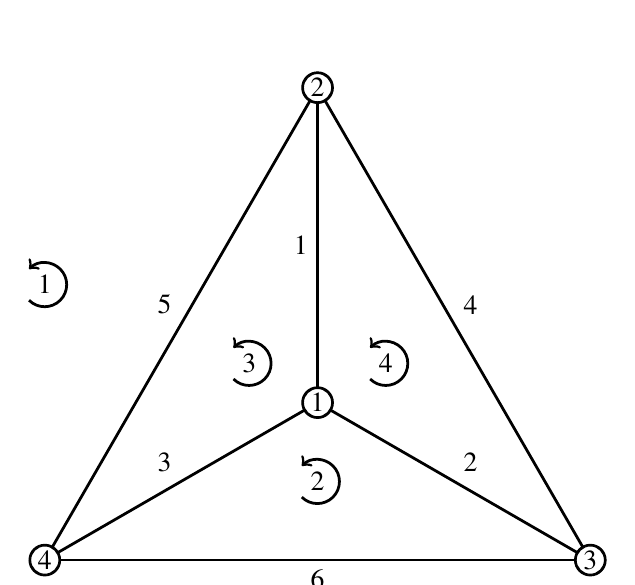
\begin{tikzpicture}[scale=4]

\coordinate (A) at (0,0);
\coordinate (B) at (0,1);
\coordinate (C) at (0.866,-0.5);
\coordinate (D) at (-0.866,-0.5);

\coordinate (b) at (0,-0.25);
\coordinate (c) at (-0.217,0.125);
\coordinate (d) at (0.217,0.125);
\coordinate (a) at (-0.866,0.375);

\coordinate (E) at (0,0.5);
\coordinate (F) at (0.433,-0.25);
\coordinate (G) at (-0.433,-0.25);
\coordinate (H) at (0.433,0.25);
\coordinate (I) at (-0.433,0.25);
\coordinate (J) at (0,-0.5);

\draw[line width=1pt] (A)--(B);
\draw[line width=1pt] (A)--(C);
\draw[line width=1pt] (A)--(D);
\draw[line width=1pt] (B)--(C);
\draw[line width=1pt] (B)--(D);
\draw[line width=1pt] (C)--(D);

\draw[fill=black] (A) circle[radius=0.5mm,fill]{};
\draw[fill=white] (A) circle[radius=0.45mm,fill]{};
\node at (A) {$1$};

\draw[fill=black] (B) circle[radius=0.5mm,fill]{};
\draw[fill=white] (B) circle[radius=0.45mm,fill]{};
\node at (B) {$2$};

\draw[fill=black] (C) circle[radius=0.5mm,fill]{};
\draw[fill=white] (C) circle[radius=0.45mm,fill]{};
\node at (C) {$3$};

\draw[fill=black] (D) circle[radius=0.5mm,fill]{};
\draw[fill=white] (D) circle[radius=0.45mm,fill]{};
\node at (D) {$4$};

\node at (b) {$2$};
\draw[->,line width=1pt] (b) + (-0.5mm,-0.5mm)
	arc[x radius=0.7mm,y radius=0.7mm,start angle=-135,end angle=135];
\node at (c) {$3$};
\draw[->,line width=1pt] (c) + (-0.5mm,-0.5mm)
	arc[x radius=0.7mm,y radius=0.7mm,start angle=-135,end angle=135];
\node at (d) {$4$};
\draw[->,line width=1pt] (d) + (-0.5mm,-0.5mm)
	arc[x radius=0.7mm,y radius=0.7mm,start angle=-135,end angle=135];
\node at (a) {$1$};
\draw[->,line width=1pt] (a) + (-0.5mm,-0.5mm)
	arc[x radius=0.7mm,y radius=0.7mm,start angle=-135,end angle=135];

\node at (E) [left] {$1$};
\node at (F) [above right] {$2$};
\node at (G) [above left] {$3$};
\node at (H) [above right] {$4$};
\node at (I) [above left] {$5$};
\node at (J) [below] {$6$};

\end{tikzpicture}
\caption{Netzwerk eines Tetraeders
\label{homologie:fig:tetragrid}}
\end{figure}

Wir berechnen die Homologie-Vektorräume für ein Tetraeder.
Ein Tetraeder besteht aus vier Dreiecken, die an den Kanten
verbunden sind.
In Abbildung~\ref{homologie:fig:tetragrid} ist das Tetraeder
schematisch dargestellt.
Die Seitenflächen sind numeriert mit den Zahlen, die von kreisförmligen
Pfeilen umgeben sind, die Seitenfläche $1$ soll man sich als die Bodenfläch
des Tetraeders vorstellen.
Die Kanten sind immer von der Ecke mit der kleineren Nummer zur
Ecke mit der grösseren Nummer orientiert.
Die Orientierung der Seitenflächen ist durch die kreisförmigen Pfeile
gegeben.

Aus dem Netzwerk~\ref{homologie:fig:tetragrid} können wir jetzt die
Randoperatoren ableiten.
Der Randoperator $\partial_1$ kann als $4\times 6$-Matrix dargestellt sind,
mit einer Zeile für jede Ecke und einer Spalte für jede Kante des
Tetraeders.
Anfangspunkte einer Kante werden mit $-1$ markiert, Endpunkte mit $1$.
So entsteht die Matrix
\[
\partial_1
=
\begin{pmatrix}
-1&-1&-1& 0& 0& 0\\
 1& 0& 0&-1&-1& 0\\
 0& 1& 0& 1& 0&-1\\
 0& 0& 1& 0& 1& 1
\end{pmatrix}.
\] 
Da die Summe jeder Spalten $0$ ist, kann $\partial_1$ nicht vollen Rang
haben.
Durch Nachrechnen findet man, dass $\operatorname{Rang}\partial_1=3$.

Der Randoperator $\partial_2$ berechnet aus jeder Seitenfläche die Summe
der orientierten Kanten, die die Seitenfläche beranden.
Wir können $\partial_2$ codieren als $6\times 4$-Matrix mit einer Zeile
für jede Kante und einer Spalte für jede Seitenfläche.
Die Kanten, die eine Seitenfläche beranden, werden mit $1$ markiert,
wenn ihre Orientierung mit der Pfeilrichtung der Seitenfläche übereinstimmt.
So erhalten wir die Matrix
\[
\partial_2
=
\begin{pmatrix}
 0& 0& 1&-1\\
 0&-1& 0& 1\\
 0& 1&-1& 0\\
 1& 0& 0&-1\\
-1& 0& 1& 0\\
 1&-1& 0& 0
\end{pmatrix}.
\]
Auch diese Matrix kann nicht vollen Rang haben, da jede Zeilensumme $0$ ist.
Tatsächlich zeigt die Rechnung dass $\operatorname{Rang}\partial_2 = 3$.

Durch Nachrechnen kann man auch kontrollieren, dass $\partial_1\partial_2=0$,
wie man das für einen Randoperator erwartet.
Daher ist $\operatorname{im}\partial_2\subset \operatorname{ker}\partial_1$.
Wir können jetzt die Dimensionen von Kern und Bild jedes Randoperators 
berechnen, und damit auch die Dimensionen der Homologie-Vektorräume.
\[
\begin{tikzcd}
	&\operatorname{dim}C_0=4
		&\operatorname{dim}C_1=6
			&\operatorname{dim}C_2=4
				&\operatorname{dim}C_3=0
\\
0
	&C_0 \ar[l,"\partial_0"]
		&C_1 \ar[l,"\partial_1"]
			&C_2 \ar[l,"\partial_2"]
				&0 \ar[l,"\partial_3"]
\\
	&{\textstyle \dim\operatorname{ker}\partial_0 = 4\atop
	 \textstyle \dim\operatorname{im}\partial_1 = 3}
		&{\textstyle\dim\operatorname{ker}\partial_1 = 3\atop
		  \textstyle\dim\operatorname{im}\partial_2 = 3}
			&{\textstyle\dim\operatorname{ker}\partial_2 = 1\atop
			  \textstyle\dim\operatorname{im}\partial_3 = 0}
\\
	&b_0=\dim H_0=1
		&b_1=\dim H_1=0
			&b_2=\dim H_2=1
\end{tikzcd}
\]
Die Bettizahlen $b_i$ führen uns auf die Euler-Charaketeristik
\[
\chi(\text{Tetraeder})
=
1 - 0 + 1 = 2,
\]
wie wir auch von der Rechnung mit dem Eulerschen Polyedersatz
aus der Einleitung dieses Abschnitts wissen.



%
% projektiv.tex
%
% (c) 2017 Prof Dr Andreas Müller, Hochschule Rapperswil
%
\subsection{Kleinsche Flasche}
Eine Kleinsche Flasche ist eine Fläche, die sich selbst durchdringt.
Die Fläche hat nur ein Seite und keinen Rand.
Wir können die Fläche mit einem Netzwerk von Dreiecken überziehen
und die Homologievektorräume berechnen oder mindestens deren Dimensionen
berechnen.
Dies ist jedoch einfacher, wenn man die Kleinsche Flasche aus einfacheren
Flächen zusammensetzen, die entsprechend einfachere Dreiecksnetze
haben.

Ein Möbius-Band entsteht, wenn man eine Streifen Papier eine halbe 
Drehung verdreht zusammenklebt.
Das Möbiusband hat nur eine Seite und nur eine Kante.
Man kann also ein Möbius-Band entlang dieses Randes mit einer
Kreisscheibe zusammenkleben.
Es stellt sich heraus, dass dadurch eine Kleinsche Flasche entsteht.
Der Plan ist also, eine Triangulation von Kreisscheibe und Möbiusband
zu finden, die am Rande zusammenpassen.
Daraus können wir dann die Randoperatoren und letztlich die Betti-Zahlen
berechnen.

\begin{figure}
\centering
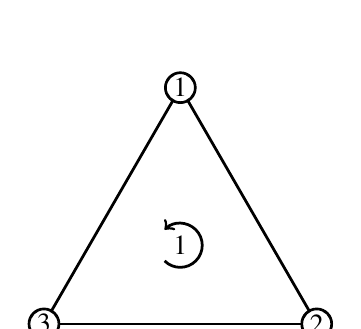
\begin{tikzpicture}[scale=4]
\coordinate (A) at (0,0.5);
\coordinate (B) at (0.433,-0.25);
\coordinate (C) at (-0.433,-0.25);
\draw[line width=1pt] (A)--(B);
\draw[line width=1pt] (A)--(C);
\draw[line width=1pt] (B)--(C);
\draw[fill=black] (A) circle[radius=0.5mm,fill]{};
\draw[fill=white] (A) circle[radius=0.45mm,fill]{};
\node at (A) {$1$};
\draw[fill=black] (B) circle[radius=0.5mm,fill]{};
\draw[fill=white] (B) circle[radius=0.45mm,fill]{};
\node at (B) {$2$};
\draw[fill=black] (C) circle[radius=0.5mm,fill]{};
\draw[fill=white] (C) circle[radius=0.45mm,fill]{};
\node at (C) {$3$};
\node at (0,0) {$1$};
\draw[->,line width=1pt] (-0.5mm,-0.5mm)
	arc[x radius=0.7mm,y radius=0.7mm,start angle=-135,end angle=135];
\end{tikzpicture}
\caption{Triangulation der Kreisscheibe
\label{homologie:fig:disk}}
\end{figure}

\begin{figure}
\centering
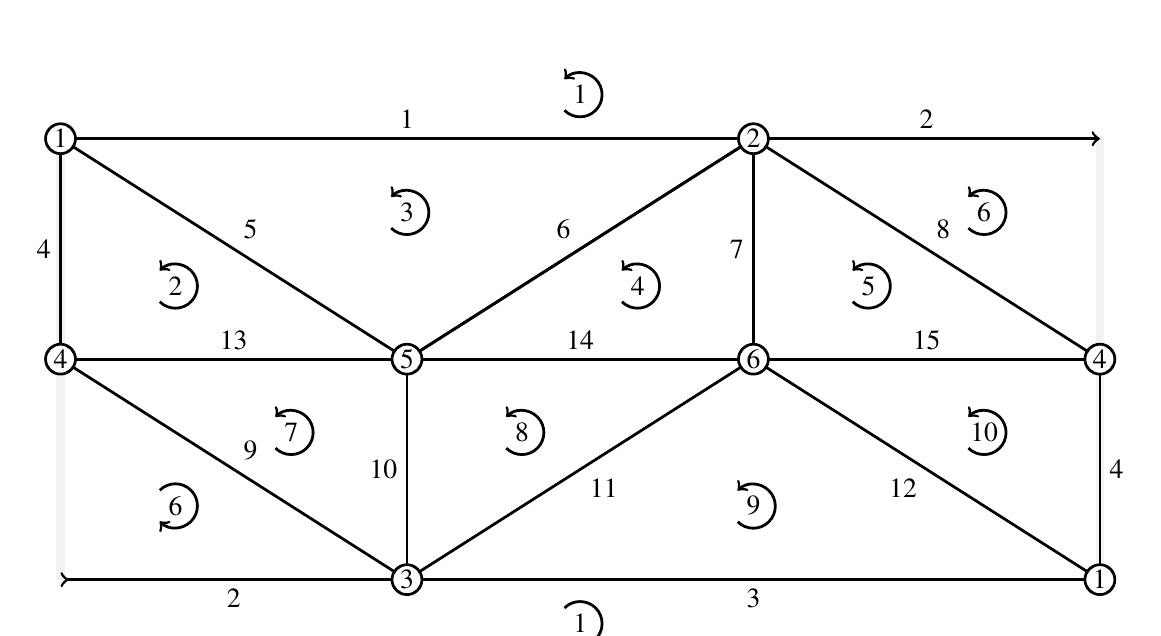
\begin{tikzpicture}[scale=4]
\def\w{2.2}
\def\h{1.4}
\coordinate (A) at ({0 * \w},{0.5 * \h});
\coordinate (a) at ({1.5 * \w},{-0.5 * \h});
\coordinate (B) at ({1 * \w},{0.5 * \h});
\coordinate (C) at ({0.5 * \w},{-0.5 * \h});
\coordinate (D) at ({0 * \w},{0 * \h});
\coordinate (E) at ({0.5 * \w},{0 * \h});
\coordinate (F) at ({1 * \w},{0 * \h});
\coordinate (d) at ({1.5 * \w},{0 * \h});
\draw[line width=3pt,color=gray!10] (A)--({0 * \w},{-0.5 * \h});
\draw[line width=3pt,color=gray!10] (a)--({1.5 * \w},{0.5 * \h});

\draw[->,line width=1pt] (A)--({1.5 * \w},{0.5 * \h});
\draw[>-,line width=1pt] ({0 * \w},{-0.5 * \h})--(a);

\draw[line width=1pt] (A)--(D);
\draw[line width=1pt] (A)--(E);
\draw[line width=1pt] (D)--(E);

\draw[line width=1pt] (B)--(E);
\draw[line width=1pt] (B)--(F);
\draw[line width=1pt] (E)--(F);

\draw[line width=1pt] (B)--(E);
\draw[line width=1pt] (B)--(d);
\draw[line width=1pt] (E)--(d);

\draw[line width=1pt] (D)--(C);
\draw[line width=1pt] (E)--(C);

\draw[line width=1pt] (C)--(F);
\draw[line width=1pt] (F)--(a);

\draw[line width=1pt] (a)--(d);

\draw[fill=black] (A) circle[radius=0.5mm,fill]{};
\draw[fill=white] (A) circle[radius=0.45mm,fill]{};
\node at (A) {$1$};

\draw[fill=black] (B) circle[radius=0.5mm,fill]{};
\draw[fill=white] (B) circle[radius=0.45mm,fill]{};
\node at (B) {$2$};

\draw[fill=black] (C) circle[radius=0.5mm,fill]{};
\draw[fill=white] (C) circle[radius=0.45mm,fill]{};
\node at (C) {$3$};

\draw[fill=black] (a) circle[radius=0.5mm,fill]{};
\draw[fill=white] (a) circle[radius=0.45mm,fill]{};
\node at (a) {$1$};

\draw[fill=black] (D) circle[radius=0.5mm,fill]{};
\draw[fill=white] (D) circle[radius=0.45mm,fill]{};
\node at (D) {$4$};

\draw[fill=black] (E) circle[radius=0.5mm,fill]{};
\draw[fill=white] (E) circle[radius=0.45mm,fill]{};
\node at (E) {$5$};

\draw[fill=black] (F) circle[radius=0.5mm,fill]{};
\draw[fill=white] (F) circle[radius=0.45mm,fill]{};
\node at (F) {$6$};

\draw[fill=black] (d) circle[radius=0.5mm,fill]{};
\draw[fill=white] (d) circle[radius=0.45mm,fill]{};
\node at (d) {$4$};

\def\flaeche#1#2{%
\node at #1 {#2};
\draw[->,line width=1pt] #1 + (-0.5mm,-0.5mm)
	arc[x radius=0.7mm,y radius=0.7mm,start angle=-135,end angle=135];
}

\def\rflaeche#1#2{%
\node at #1 {#2};
\draw[->,line width=1pt] #1 + (-0.5mm,0.5mm)
	arc[x radius=0.7mm,y radius=0.7mm,start angle=135,end angle=-135];
}

\flaeche{({0.166*\w},{0.166*\h})}{$2$};
\flaeche{({0.5*\w},{0.333*\h})}{$3$};
\flaeche{({0.833*\w},{0.166*\h})}{$4$};
\flaeche{({1.166*\w},{0.166*\h})}{$5$};
\flaeche{({1.333*\w},{0.333*\h})}{$6$};
\flaeche{({0.333*\w},{-0.166*\h})}{$7$};
\flaeche{({0.666*\w},{-0.166*\h})}{$8$};
\flaeche{({1*\w},{-0.333*\h})}{$9$};
\flaeche{({1.333*\w},{-0.166*\h})}{$10$};

\rflaeche{({0.166*\w},{-0.333*\h})}{$6$};
%\node at ({0.166*\w},{-0.333*\h}) {$6$};
%\draw[->,line width=1pt]
%	({0.166*\w},{-0.333*\h}) +(-0.5mm,0.5mm)
%	arc[x radius=0.7mm,y radius=0.7mm,start angle=135,end angle=-135];

\flaeche{({0.75*\w},{0.6*\h})}{$1$};
\rflaeche{({0.75*\w},{-0.6*\h})}{$1$};

\node at ({0.5*\w},{0.5*\h}) [above] {$1$};
\node at ({1.25*\w},{0.5*\h}) [above] {$2$};
\node at ({1*\w},{-0.5*\h}) [below] {$3$};
\node at ({0.25*\w},{-0.5*\h}) [below] {$2$};

\node at ({0*\w},{0.25*\h}) [left] {$4$};
\node at ({0.25*\w},{0.25*\h}) [above right] {$5$};
\node at ({0.75*\w},{0.25*\h}) [above left] {$6$};
\node at ({1*\w},{0.25*\h}) [left] {$7$};
\node at ({1.25*\w},{0.25*\h}) [above right] {$8$};

\node at ({0.25*\w},{-0.25*\h}) [above right] {$9$};
\node at ({0.5*\w},{-0.25*\h}) [left] {$10$};
\node at ({0.75*\w},{-0.25*\h}) [below right] {$11$};
\node at ({1.25*\w},{-0.25*\h}) [below left] {$12$};
\node at ({1.5*\w},{-0.25*\h}) [right] {$4$};

\node at ({0.25*\w},0) [above] {$13$};
\node at ({0.75*\w},0) [above] {$14$};
\node at ({1.25*\w},0) [above] {$15$};

\end{tikzpicture}
\caption{Triangulation des Möbisubandes
\label{homologie:fig:moebius}}
\end{figure}

\subsubsection{Triangulation der Kleinschen Flasche}
Die Kreisscheibe können wir als einfaches Dreieck triangulieren, wie
es in Abbildung~\ref{homologie:fig:klein} dargestellt ist.
Wie in früheren Beispielen sind die Kanten von kleineren Eckennummern
zu grösseren Eckennummern orientiert.
Das Möbiusband ist etwas komplizierter zu triangulieren.
Eine Möglichkeit ist in Abbildung~\ref{homologie:fig:klein} dargestellt.


\subsubsection{Randoperatoren}
Die Randoperatoren für die Kleinsche Flasche können jetzt aus
den Abbildungen \ref{homologie:fig:disk} und \ref{homologie:fig:moebius}
abgelesen werden.
Den $15$ Kanten werden jeweils zwei der $6$ Ecken zugeordnet, wie
durch die Matrix
\[
\setcounter{MaxMatrixCols}{15}
\partial_1
=
\begin{pmatrix}
%1  2  3  4  5  6  7  8  9 10 11 12 13 14 15
-1& 0&-1&-1&-1& 0& 0& 0& 0& 0& 0&-1& 0& 0& 0\\
 1&-1& 0& 0& 0&-1&-1&-1& 0& 0& 0& 0& 0& 0& 0\\
 0& 1& 1& 0& 0& 0& 0& 0&-1&-1&-1& 0& 0& 0& 0\\
 0& 0& 0& 1& 0& 0& 0& 1& 1& 0& 0& 0&-1& 0&-1\\
 0& 0& 0& 0& 1& 1& 0& 0& 0& 1& 0& 0& 1&-1& 0\\
 0& 0& 0& 0& 0& 0& 1& 0& 0& 0& 1& 1& 0& 1& 1
\end{pmatrix}
\]
beschrieben.
Der Randoperator $\partial_2$ ordnet jeder der Seitenfläche eine Summe
von Kanten zu mit positivem Vorzeichen jeweils dann, wenn die Kante gleich
orientiert ist wie der Pfeil der Seitenfläche anzeigt.
Die so definiert $15\times 10$-Matrix ist
\[
\partial_2
=
\begin{pmatrix}
%1  2  3  4  5  6  7  8  9 10
 1& 0&-1& 0& 0& 0& 0& 0& 0& 0	\\ %  1
 1& 0& 0& 0& 0&-1& 0& 0& 0& 0	\\ %  2
-1& 0& 0& 0& 0& 0& 0& 0&-1& 0	\\ %  3
 0& 1& 0& 0& 0& 0& 0& 0& 0& 1	\\ %  4
 0&-1& 1& 0& 0& 0& 0& 0& 0& 0	\\ %  5
 0& 0&-1& 1& 0& 0& 0& 0& 0& 0	\\ %  6
 0& 0& 0&-1& 1& 0& 0& 0& 0& 0	\\ %  7
 0& 0& 0& 0&-1& 1& 0& 0& 0& 0	\\ %  8
 0& 0& 0& 0& 0&-1&-1& 0& 0& 0	\\ %  9
 0& 0& 0& 0& 0& 0& 1&-1& 0& 0	\\ % 10
 0& 0& 0& 0& 0& 0& 0& 1&-1& 0	\\ % 11
 0& 0& 0& 0& 0& 0& 0& 0& 1&-1	\\ % 12
 0& 1& 0& 0& 0& 0&-1& 0& 0& 0	\\ % 13
 0& 0& 0& 1& 0& 0& 0&-1& 0& 0	\\ % 14
 0& 0& 0& 0&-1& 0& 0& 0& 0& 1	\\ % 15
\end{pmatrix}
\]
Beide Operatoren haben nicht vollen Rang, die Berechnung ergibt
\[
\operatorname{Rang}\partial_1 = 5
\qquad\text{und}\qquad
\operatorname{Rang}\partial_2 = 10.
\]
Durch Nachrechnen überprüft man auch $\partial_1\partial_2=0$, also
$\operatorname{im}\partial_2\subset \operatorname{ker}\partial_1$.

\subsubsection{Homologie einer Kleinschen Flasche}
Aus den bekannten Randoperatoren $\partial_1$ und $\partial_2$ kann
man jetzt die Dimensionen der Homologievektorräume berechnen:
\[
\begin{tikzcd}
	&\operatorname{dim}C_0 = 6
		&\operatorname{dim}C_1 = 15
			&\operatorname{dim}C_2 = 10
				&
\\
0
	&C_0 \ar[l,"\partial_0"]
		&C_1 \ar[l,"\partial_1"]
			&C_2 \ar[l,"\partial_2"]
				&0
\\
	&{\textstyle\dim\operatorname{ker}\partial_0=6\atop
	  \textstyle\dim\operatorname{im}\partial_1=5}
		&{\textstyle\dim\operatorname{ker}\partial_1=10\atop
		  \textstyle\dim\operatorname{im}\partial_2=10}
			&{\textstyle\dim\operatorname{ker}\partial_2=0\atop
			  \textstyle\dim\operatorname{im}\partial_3=0}
\\
	&\dim H_0 = 1
		&\dim H_1 = 0
			&\dim H_2 = 0
\end{tikzcd}
\]
Aus sicht der reellen Homologie-Vektorräume ist die Kleinsche Flasche
also nicht von einem Punkt unterscheidbar.
Betrachtet man allerdings alle Vektorräume als Vektorräume über
$\mathbb F_2$, dann ergibt sich ein anderes Bild.
In den Matrizen $\partial_1$ und $\partial_2$ ist dann $-1$ durch $1$
zu ersetzen.
Die Berechnung des Ranges ergibt
\[
\operatorname{Rang}\partial_1 = 5
\qquad\text{und}\qquad
\operatorname{Rang}\partial_2 = 9
\]
Die Dimensionen der Homologie-Vektorräume sind
\[
\begin{tikzcd}
	&\operatorname{dim}C_0 = 6
		&\operatorname{dim}C_1 = 15
			&\operatorname{dim}C_2 = 10
				&
\\
0
	&C_0 \ar[l,"\partial_0"]
		&C_1 \ar[l,"\partial_1"]
			&C_2 \ar[l,"\partial_2"]
				&0
\\
	&{\textstyle\dim\operatorname{ker}\partial_0=6\atop
	  \textstyle\dim\operatorname{im}\partial_1=5}
		&{\textstyle\dim\operatorname{ker}\partial_1=10\atop
		  \textstyle\dim\operatorname{im}\partial_2=9}
			&{\textstyle\dim\operatorname{ker}\partial_2=1\atop
			  \textstyle\dim\operatorname{im}\partial_3=0}
\\
	&\dim H_0 = 1
		&\dim H_1 = 1
			&\dim H_2 = 1
\end{tikzcd}
\]
Der Unterschied stammt daher, dass die $\mathbb F_2$-Homologie zwischen
$1$ und $-1$ nicht unterschieden kann, also die Orientierung der
Flächen und Kanten ignoriert.
Die $\mathbb R$-Homologie dagegen kann die beiden Orientierungen
unterschieden.







%
% algtopo.tex -- Intro in die algebraische Topologie
%
% (c) 2017 Prof Dr Andreas Müller, Hochschule Rapperswil
%
\section{Algebraische Topologie}
\rhead{Algebraische Topologie}
Die in diesem Kapitel gezeigte elementare Homologietheorie ist ein
erster Schritt in das weite Gebiet der algebraischen Topologie.
Diese befasst sich mit den Eigenschaften geometrischer Objekte, die
sich unter Deformationen nicht ändern.
Das Grundprinzip ist, einem geometrischen Objekt ein algebraisches Objekt
zuzuordnen.
Zum Beispiel haben wir gesehen, wie man einem Polyeder oder allgemeiner
einem simplizialen Komplex $X$ eine Reihe von Vektorräumen $H_0(X,\mathbb R)$,
$H_1(X,\mathbb R),\dots$ zuordnet.
An verschiedenen Dimensionen dieser Vektorräume können wir bereits 
Unterschiede erkennen.

Die Dimension des Homologie-Vektorraumes $H_0(X,\mathbb R)$ gibt die Anzahl
der Zusammenhangskomponenten an.
Die Dimension von $H_1(X,\mathbb R)$ zählt die Zyklen, die 








%
% lie.tex -- Lie Gruppen und Lie Algebrean
%
% (c) 2017 Prof Dr Andreas Müller, Hochschule Rapperswil
%
\chapter{Lie Gruppen und Lie Algebren}
\rhead{Lie Gruppen und Lie Algebren}
Im Skript werden einige spezielle Matrizengruppen untersucht,
zum Beipsiel die Gruppen $\textrm{SO}(2)$ und $\textrm{SO}(3)$.
Von Lie stammt eine allgemein Theorie solcher Gruppen, die für die
Anwendungen von grosser Bedeutung ist.
In diesem Kapitel werden die grundlegenden Eigenschaften von 
Lie Gruppen und Lie Algebren an weitern Beispielen zusammengetragen.

\section{Lie Gruppen}

\section{Lie Algebren}

\section{Die Drehgruppe $\textrm{SO}(3)$}

\subsection{Infinitesimale Drehungen des $\mathbb R^3$}

\subsection{Lie Algebra $\textbf{so}(3)$ und Vektorprodukt}


%
% part2.tex -- Beweis
%
% (c) 2017 Prof Dr Andreas Müller, Hochschule Rapperswil
%
\part{Beweis}

\chapter*{Beweis in der Mathematik}
Die Mathematik zeichnet sich gegenüber den Naturwissenschaften dadurch
aus, dass sie absolute Wahrheiten verkündet. 
Aber tut sie das wirklich?
In diesem Kapitel sollen die Fragen der Grundlagen der Mathematik
erläutert werden an einigen interessanten Aspekten, die für die lineare
Algebra relevant sind.


\input nichtstandardanalysis.tex
%
% part3.tex -- Berechnung
%
% (c) 2017 Prof Dr Andreas Müller, Hochschule Rapperswil
%
\part{Berechnung}

\chapter*{Numerische lineare Algebra}
In einer Grundlagen-Vorlesung über lineare Algebra werden meistens nur
die einfachsten numerischen Methoden besprochen.
Natürlich gehört der Gauss-Algorithmus dazu, doch seine Komplexität
von $O(n^3)$ ist für viele Anwendungen viel zu schlecht.
Zum Beispiel treten bei Anwendungen mit finiten Elementen sehr grosse
Gleichungssysteme auf, die jedoch oft eine besondere Struktur haben.
Daher wurden besondere Algorithmen geschaffen, mit denen auch solche
Gleichungssysteme gelöst werden können.







\input pca.tex
\vfill
\pagebreak
\ifodd\value{page}\else\null\clearpage\fi
\input supplement.ind
\appendix
\end{document}
